\documentclass[]{politex}
% ========== Opções ==========
% pnumromarab - Numeração de páginas usando algarismos romanos na parte pré-textual e arábicos na parte textual
% abnttoc - Forçar paginação no sumário conforme ABNT (inclui "p." na frente das páginas)
% normalnum - Numeração contínua de figuras e tabelas 
%	(caso contrário, a numeração é reiniciada a cada capítulo)
% draftprint - Ajusta as margens para impressão de rascunhos
%	(reduz a margem interna)
% twosideprint - Ajusta as margens para impressão frente e verso
% capsec - Forçar letras maiúsculas no título das seções
% espacosimples - Documento usando espaçamento simples
% espacoduplo - Documento usando espaçamento duplo
%	(o padrão é usar espaçamento 1.5)
% times - Tenta usar a fonte Times New Roman para o corpo do texto
% noindentfirst - Não indenta o primeiro parágrafo dos capítulos/seções


% ========== Packages ==========
\usepackage[utf8]{inputenc}
\usepackage{amsmath,amsthm,amsfonts,amssymb}
\usepackage{graphicx,cite,enumerate}
\usepackage{float}
\usepackage{t1enc}
\usepackage{array}
\usepackage[num]{abntex2cite}
\usepackage{longtable}
\usepackage{multirow}
\usepackage{caption}
% \usepackage{floatrow}

% ========== Language options ==========
\usepackage[brazil]{babel}
%\usepackage[english]{babel}


% ========== ABNT (requer ABNTeX 2) ==========
%	http://www.ctan.org/tex-archive/macros/latex/contrib/abntex2
%\usepackage[num]{abntex2cite}

% Forçar o abntex2 a usar [ ] nas referências ao invés de ( )
%\citebrackets{[}{]}


% ========== Lorem ipsum ==========
\usepackage{blindtext}
\graphicspath{ {images/} }


% ========== Opções do documento ==========
% Título
\titulo{Monitoramento Inteligente de Ambientes com foco no bem-estar}

% Autor
\autor{Adilson Torres Gregório de Souza \\
       Jhonata Antunes}

% Para múltiplos autores (TCC)
%\autor{Nome Sobrenome\\%
%		Nome Sobrenome\\%
%		Nome Sobrenome}

% Orientador / Coorientador
\orientador{Prof. Dr. Reginaldo Arakaki}
\coorientador{Prof. Dr. Jorge Luis Risco Becerra}

% Tipo de documento
%\tcc{Eletricista com ênfase em Sistemas Eletrônicos}
\tcc{Engenharia Computação}
%\teseDOC{Engenharia Elétrica}
%\teseLD
%\memorialLD

% % Departamento e área de concentração
\departamento{PCS}
\areaConcentracao{Engenharia Computação}

% Local
\local{São Paulo}

% Ano
\data{2018}




\begin{document}
% ========== Capa e folhas de rosto ==========
\capa
\falsafolhaderosto
\folhaderosto


% ========== Folha de assinaturas (opcional) ==========
% \begin{folhadeaprovacao}
% 	\assinatura{Prof.\ X}
% 	\assinatura{Prof.\ Y}
% 	\assinatura{Prof.\ Z}
% \end{folhadeaprovacao}
% ========== Folha de assinaturas (opcional) ==========
\begin{folhadeaprovacao}
\noindent
Nome: SOUZA, Adilson Torres Gregório de\\
Nome: ANTUNES, Jhonata

\noindent
Título: Monitoramento inteligente de ambientes com foco no bem-estar

\vspace{1cm}
\hspace{.2\textwidth} % posicionando a minipage 
\begin{minipage}{.75\textwidth}
  \begin{espacoumemeio}
    \begin{sloppypar}
        Monografia (Trabalho de Conclusão de Curso) apresentada à Escola Politécnica da Universidade de São Paulo para a obtenção do Título de Bacharel em Engenharia na área de Engenharia de Computação. \\[0.3cm]
    \end{sloppypar}
  \end{espacoumemeio}
\end{minipage} 
    
%\noindent
%Aprovada em: 
\noindent
Trabalho entregue para o departamento em: \\

\begin{center}
%Banca Examinadora
Responsáveis
\end{center}

\assinatura{Prof. Dr. Reginaldo Arakaki (Orientador)}

\assinatura{Prof. Dr. Jorge Luis Risco Becerra (Co-orientador)}

\assinatura{Adilson Torres Gregório de Souza (Orientado)}

\assinatura{Jhonata Antunes (Orientado)}
\end{folhadeaprovacao}
% ========== Ficha catalográfica ==========
% Fazer solicitação no site:
%	http://www.poli.usp.br/en/bibliotecas/servicos/catalogacao-na-publicacao.html


% ========== Dedicatória (opcional) ==========
% \dedicatoria{Dedicatória}


% ========== Agradecimentos ==========
% \begin{agradecimentos}

% Obrigado...

% \end{agradecimentos}


% ========== Epígrafe (opcional) ==========
%\epigrafe{%
%	\emph{``Epígrafe''}
%	\begin{flushright}
%		-{}- Autor
%	\end{flushright}
%}


% ========== Resumo ==========
\begin{resumo}
Resumo...

\\[3\baselineskip]

\textbf{Palavras-Chave} -- Palavra, Palavra, Palavra, Palavra, Palavra.
\end{resumo}


% ========== Abstract ==========
\begin{abstract}
Abstract...

\\[3\baselineskip]

\textbf{Keywords} -- Word, Word, Word, Word, Word.
\end{abstract}


% ========== Listas (opcional) ==========
\listadefiguras
\listadetabelas

% ========== Listas definidas pelo usuário (opcional) ==========


% ========== Sumário ==========
\sumario



% ========== Elementos textuais ==========

% \part{Introdução}
	
\chapter{Introdução}
% \capepigrafe[0.5\textwidth]{``Frase espirituosa de um autor famoso''}{Autor famoso}
\section{Motivação}
Com o avanço da tecnologia, as antigas câmeras analógicas estão sendo substituídas pelas câmeras IP, que são melhores em termos de resolução, visão noturna, entre outras características. O barateamento da tecnologia e problemas sociais, como segurança, levaram a um acentuado aumento na quantidade de câmeras distribuídas por todo o mundo. Na área de monitoramento, elas são utilizadas, na maior parte, como um recurso auxiliador.  “Elas não substituem o guarda, simplesmente são uma ferramenta muito importante de apoio" (\citeauthoronline{bermudez}, \citeyear{bermudez}).

O desenvolvimento de estudos e tecnologias na área de inteligência artificial possibilitou que alguns sistemas aplicassem inteligência ao monitoramento, como o ShotSpotter. Esse sistema é capaz de detectar precisamente a posição de um disparo de arma de fogo. Primeiro, softwares especializados analisam sinais de áudio para determinar potenciais disparos de arma de fogo; depois, o software determina a localização da fonte do áudio e analisa as características do som para determinar se é parecido com um disparo; em caso positivo, envia alertas para a polícia e equipes de emergência (\citeauthoronline{shotspooter}, \citeyear{shotspooter}).

Na área de monitoramento inteligente por análise de vídeos, existe uma patente registrada na Oficina de Patentes Europeia, de número AU2018100039, que propõem soluções para o problema de segurança. O sistema identifica e rastreia pessoas que causam ameaça a segurança pública, incluindo determinação de rotas de fuga para longe da ameaça (\citeauthoronline{patente}, \citeyear{patente}).

Os sistemas de monitoramento comuns, por vídeos de vigilância, são amplamente empregados, servindo como ferramenta auxiliar, e, pelo fato de ser analisado por um operador humano, possui múltiplas funções, porém, é pouco eficiente, pois requer muito trabalho manual. Os sistemas inteligentes, por sua vez, são eficientes e escaláveis, porém, ainda estão pouco desenvolvidos. Não há nenhum sistema específico que use monitoramento inteligente baseado em vídeos para detectar eventos, focados no bem estar, e prestar assistência, quando necessário.

\section{Objetivo}
O objetivo deste trabalho é desenvolver a arquitetura de um sistema de Monitoramento Inteligente de Ambientes que seja capaz de processar imagens recebidas de câmeras para detectar eventos, relacionados ao bem estar das pessoas presentes no ambiente, e realizar um conjunto de ações específicas para cada evento. O sistema deve receber as imagens, utilizar técnicas de inteligência artificial para reconhecer objetos, aplicar algoritmos detectores de eventos e, quando detectado um evento, tomar um conjunto de ações. Os eventos estão relacionados ao bem estar das pessoas, portanto, podem ser acidente de trânsito, assalto à mão armada, desmaio, incêndio, agressão física, entre outros. As ações dependem diretamente do evento, e podem ser acionar polícia, corpo de bombeiros, ambulância e, dependendo do nível de integração disponível, acionar semáforos para isolar áreas ou, até mesmo, acionar robôs ou dispositivos de prestação de ajuda para atuarem no local do evento.

\section{Justificativa}
O rápido desenvolvimento da tecnologia das câmeras as tornou o principal meio de realizar o monitoramento de ambientes, porém, o mesmo não ocorreu com as ferramentas de monitoramento, de forma que as imagens são utilizadas como apoio, em vez de serem o ponto central, não aproveitando o grande potencial de informação que elas possuem e dificultando tomadas de decisão em tempo real em sistemas de larga escala.

Sistemas como o ShotSpotter iniciam a caminhada rumo a ferramentas de monitoramento inteligente, porém, esse sistema, em específico, além de detectar apenas um tipo de evento, depende da instalação de sensores de áudio, de forma a reduzir a aplicabilidade do sistema. Para contornar esse problema, é preciso desenvolver um sistema cuja principal fonte de dados já esteja difundida em diversos ambientes. Essa fonte de dados é o vídeo das câmeras, onde seu uso vem aumentando constantemente.

Alguns eventos, como acidentes, requerem que as vítimas sejam atendidas o mais rápido possível, contudo, em locais pouco movimentados, pode ser difícil que alguma pessoa detecte o evento, determinar o local do evento ou acionar a ajuda. Portanto, é necessário um sistema que seja capaz de detectar eventos em tempo real, para realizar as ações necessárias para prestar assistência o quanto antes. Para aumentar a área de atuação do sistema, é preciso utilizar um mecanismo de observação que já esteja bem difundido nos diversos tipos de ambientes, como vídeos de vigilância.


\section{Organização do trabalho}
A seção 2 aborda os aspectos conceituais necessários para o desenvolvimento do trabalho, tendo para cada conceito e técnica utilizado uma breve explicação, tais como processamento de imagens, \textit{machine learning} e  RM-ODP. Na seção 3 é descrito com mais detalhes as principais tecnologias utilizadas. Na seção 4 é apresentado a metodologia utilizada no trabalho, com gerenciamento de tarefas, versionamento git e pesquisas realizadas. Na seção 5 é detalhado a especificação do projeto. Na seção 6, documentou o estudo, implementação e resultados dos testes. Na seção 7, é documentado os testes e avaliações da implementação. Na seção 8, é apresentado as considerações finais do trabalho.

\chapter{Aspectos Conceituais}

\section{Processamento de imagens}
\subsection{Equalização de histogramas} \label{histogramas}
Histograma é a distribuição de frequências de um certo fenômeno ou característica, que pode ser representado visualmente por gráficos de colunas ou barras. Assim sendo, o histograma de uma imagem representa a distribuição de frequência dos componentes de cor. Para cores representadas com 8 bits, a abscissa varia de 0 a 255, representando a intensidade de um canal de cor, e a coordenada representa a quantidade de pixels de uma certa intensidade de cor.

Quando um certo ambiente não possui iluminação equilibrada, a imagem capturada pode ter uma alta frequência de pixels com intensidade de cor próximas, como no primeiro histograma da Figura \ref{fig:opencv_histograma}. Isto é característico de imagens com pouco contraste de cores. A equalização de histogramas é uma operação que distribui as frequências para ambas as extremidades do gráfico. Imagens com as intensidades de cores melhor distribuídas apresentam um bom contraste.

O contraste é uma característica que evidencia os limites e bordas dos objetos contidos nas imagens, pois há uma variação brusca de cores. Essa característica é muito positiva para algoritmos detectores de objetos que se baseiam no contorno dos objetos.

\begin{figure}[H]
    \centering
    \caption{Exemplo do resultado da operação de equalização de histogramas}
    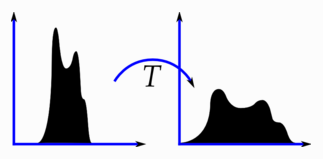
\includegraphics[width=0.8\textwidth]{opencv_histograma}
    \caption*{Fonte: (\citeauthoronline{opencvtutorials}, \citeyear{opencvtutorials})}
    \label{fig:opencv_histograma}
\end{figure}

\subsection{Convolução matricial}
No contexto de redes neurais, a convolução de matrizes, também referenciada apenas como convolução, é uma operação que empenha um importante papel no funcionamento de redes neurais convolucionais. Sua importância se dá pelo fato de que tal operação permite extrair características das imagens, como bordas, relevo, entre outras. Essa extração de características é fundamental para as redes neurais que detectam objetos.

O processo de convolução consiste em uma matriz \(E_{n \times m}\) e um filtro \(F_{f \times f}\), onde o filtro se sobrepõe a matriz de entrada, calcula um valor de saída, desliza para a posição seguinte e repete os passos seguintes até que o filtro tenha se sobreposto a todas as regiões possíveis (ver Figura \ref{fig:convolucao}). O cálculo do valor de saída de cada sobreposição é dado pela soma dos produtos dos valores sobrepostos da matriz de entrada e do filtro, como exemplificado na Figura \ref{fig:convolucao}. As dimensões da matriz de saída é dado por \( (n-f+1) \times (m-f+1)\) (\citeauthoronline{cnncourse}, \citeyear{cnncourse}).

\begin{figure}[H]
    \centering
    \caption{Exemplo simples de convolução}
    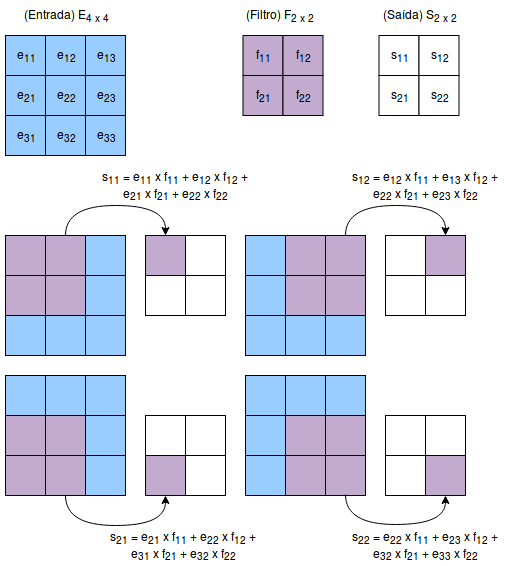
\includegraphics[width=0.8\textwidth]{Convolucao}
    \caption*{Fonte: Autores}
    \label{fig:convolucao}
\end{figure}

\subsubsection{Padding}
A convolução normal leva em consideração muito fracamente os valores das bordas da imagem, enquanto que os centrais, são utilizados mais de uma vez no cálculo de um valor do \textit{feature map}. Para contornar esse problema, dando maior expressividade aos pixels da borda, é possível adicionar um \textit{padding}, ou seja, envolver a imagem com pixels de valor nulo. Vale notar que os filtros geralmente (é possível observar na literatura) tem tamanho ímpar. Seja uma imagem de tamanho \(n \times m\), \textit{padding} \(p\) e um filtro \(f \times f\), então, a matriz resultante (\textit{feature map}) terá tamanho \((n+2p-f+1) \times (m+2p-f+1)\) (\citeauthoronline{cnncourse}, \citeyear{cnncourse}).

\subsubsection{Strided convolution}
\textit{Strided convolution} é uma convolução com um passo maior que um, ou, uma convolução normal é aquela onde \(stride=1\) (passo igual a um). O passo se refere a quantos pixels deve se deslocar (horizontal e verticalmente) o filtro sobre a imagem. Dessa forma, realizando um salto maior com o filtro sobre a imagem, os pixels serão considerados em menos valores da feature map resultante. Isso diminui a precisão da extração de características, porém, reduz o tamanho da saída (\textit{feature map}), diminuindo o processamento e consumo de memória da rede neural, que pode utilizar diversos filtros ao mesmo tempo. A convolução de uma imagem de tamanho \(n \times m\) e um filtro \(f \times f\), com \textit{padding} \(p\) e \textit{stride} \(s\) resulta em uma matriz de tamanho \((\frac{n+2p-f}{s}+1) \times (\frac{m+2p-f}{s}+1)\) (\citeauthoronline{cnncourse}, \citeyear{cnncourse}).

\subsubsection{Pooling}
Pooling é um tipo de técnica amplamente utilizada nas camadas das redes neurais convolucionais. Ela consiste em escolher um tamanho de janela de tamanho \(f \times f\), um passo \(s\), e deslizar a janela sobre a imagem. O processo é similar ao de convolução, onde a diferença está na computação do resultado. Os parâmetros \(f\) e \(s\) não participam do processo de aprendizagem, e são chamados de hiper-parâmetros, pois não existe uma regra para a definição de seus valores (\citeauthoronline{cnncourse}, \citeyear{cnncourse}). A seguir, os dois tipos de \textit{pooling} mais utilizados:
\begin{itemize}
\item \textit{Max pooling}: consiste em escolher o máximo valor dentro da janela;
\item \textit{Average pooling}: consiste em calcular o valor médio dos valores da janela.
\end{itemize}

\section{Machine Learning}
\subsection{Redes Neurais}
Os resultados dos estudos da neurociência assumem como hipótese que as atividades mentais consistem, primariamente, em atividades eletroquímicas nas redes de células do cérebro, chamadas neurônios (\citeauthoronline{Russell}, \citeyear{Russell}). Inspirados nesses princípios, foram desenvolvidos modelos matemáticos do cérebro humano, de forma a gerar grandes contribuições à área de inteligência artificial, através das redes neurais artificiais.

\subsubsection{Neurônio artificial}
O neurônio artificial é um modelo matemático do neurônio cerebral. Ele consiste em múltiplas ligações de entrada, uma função de ativação e uma ligação de saída, como ilustrado na Figura \ref{fig:neuronio}.

\begin{figure}[H]
    \centering
    \caption{Modelo matemático de um neurônio simples. A saída da unidade é \(a_j\), onde \(a_i\) é a saída da unidade \(i\) e \(w_{ij}\) é o peso das ligações da unidade \(i\) para esta unidade.}
    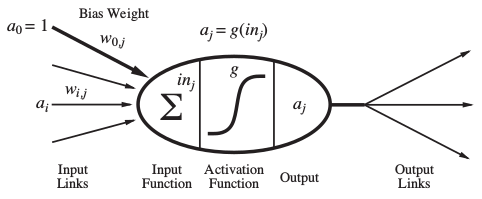
\includegraphics[width=0.8\textwidth]{Neuronio}
    \caption*{Fonte: (\citeauthoronline{Russell}, \citeyear{Russell})}
    \label{fig:neuronio}
\end{figure}

As ligações de entrada tem a importante característica de possuir pesos. Cada ligação possui seu valor numérico de peso, de forma que cada uma é percebida com uma certa importância.

A função de ativação é, tipicamente, do tipo limite rígido (\textit{hard threshold}) ou função logística (\textit{logistic function}). No primeiro caso, a unidade é chamada de \textit{perceptron} e no segundo, \textit{sigmoid perceptron}. Essas duas funções garantem a importante propriedade de que a rede, como um todo, pode representar uma função não linear. A vantagem de usar a função logística é que ela é diferenciável em todo seu domínio (\citeauthoronline{Russell}, \citeyear{Russell}).

\begin{figure}[H]
    \centering
    \caption{(a) \textit{hard threshold function} e (b)\textit{ logistic function}}
    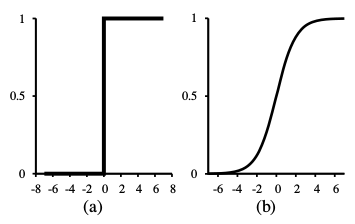
\includegraphics[width=0.6\textwidth]{funcativacao}
    \caption*{Fonte: (\citeauthoronline{Russell}, \citeyear{Russell})}
    \label{fig:funcativacao}
\end{figure}

\subsubsection{Estrutura das redes neurais}
Uma vez definidos os modelos matemáticos do neurônio, é preciso conectá-los, para formar uma rede. Há duas formas fundamentais de realizar esta tarefa, onde a primeira é conhecida como \textit{feed-forward network} e a segunda, \textit{recurrent network}.

As \textit{feed-forward network} possuem conexão em apenas uma direção, de modo a formar um grafo não cíclico. Todo nó recebe como entrada dados dos nós anteriores, e passam dados para os nós posteriores, sem formar laços (\citeauthoronline{Russell}, \citeyear{Russell}). Este tipo de rede é uma função apenas dos valores de entrada, onde não há estados internos.

As \textit{recurrent network} possuem conexões em ambas as direções, de modo que a saída de nós posteriores podem ser entrada de nós anteriores (\citeauthoronline{Russell}, \citeyear{Russell}). Este tipo de rede é uma função dos valores de entrada e dos estados internos. Dessa forma, uma característica importante deste tipo de rede é que ela passou memória de curto prazo, sendo um modelo mais próximo do cérebro humano. Uma de suas desvantagens é que a alta complexidade e o fato de que o modelo pode alcançar estados caóticos, apresentar oscilações ou comportamento caótico.

\subsubsection{Rede neural convolucional}
Rede neural convolucional é um tipo de rede neural artificial que é composta por camadas de convolução (convolucional layers) e redes completamente conectadas (\textit{fully connected layers}). Ela é uma rede do tipo \textit{feed-forward network} e pode conter \textit{skip connections}, que consiste em ligar a saída de uma camada à entrada de outra camada cuja distância é maior que um. Sua maior aplicação está na área de processamento de imagens, devido ao fato de possuir grande eficiência em extração de características (\textit{feature extraction}) de imagens, fornecida pelas camadas convolucionais.

As \textit{convolucional layers} são, geralmente, as primeiras da rede, seguidas das \textit{fully connected layers}. Elas são compostas por convolução do tipo normal, \textit{strided convolution}, \textit{max pooling} e \textit{average pooling}. Uma característica importante das convolucional layers é que diversos filtros podem ser aplicados em uma mesma camada, de forma que a dimensão dos dados diminui ao longo das camadas, enquanto que a profundidade aumenta.

As \textit{fully connected layer}s são camadas de rede neural formadas por neurônios completamente conectados, ou seja, a saída de um nó é uma das entradas de todos os nós da camada posterior. Essas camadas são utilizadas geralmente para codificar os dados de saída.

\begin{figure}[H]
    \centering
    \caption{Exemplo de CNN do YOLO v1, que contém 24 \textit{convolucional layers} e 2 \textit{fully connected layers}}
    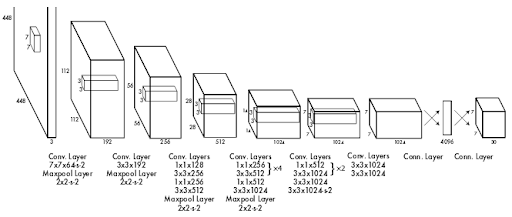
\includegraphics[width=\textwidth]{arquitetura_yolo}
    \caption*{Fonte: (\citeauthoronline{yolov1}, \citeyear{yolov1})}
    \label{fig:arq_yolo}
\end{figure}

\subsection{IoU}
IoU (\textit{Intersection over Union}) ou também conhecido como índice de Jaccard é uma medida de similaridade em conjuntos. Na área de \textit{machine learning} é utilizado como uma medida de acurácia de um detector de objetos em um dado \textit{dataset}. O cálculo é feito através de duas áreas, a primeira área é considerado um retângulo sobre o objeto a ser detectado e a segunda área o retângulo predito pelo detector de objetos. Com essas duas áreas o cálculo do IoU se torna a área de intersecção entre as áreas dos retângulos sobre a área de união dos retângulos, valores abaixo de 0.5 são considerados de baixa qualidade enquanto que valores perto de 1 são considerados adequados (\citeauthoronline{iou}, \citeyear{iou}).

\subsection{NMS (Non-Maximum Suppresion)}
NMS (\textit{Non-Maximum Suppression}) é um algoritmo de pós processamento de imagem responsável por agrupar as detecções feitas sobre um mesmo objeto. Um detector de objetos possui essencialmente 3 passos, o primeiro é propor um espaço de buscas em janelas, o segundo é pontuar e refinar cada janela com um classificador ou regressor, e o último passo é juntar as janelas quando estas pertencem a um mesmo objeto, este último passo é feito através do NMS. Ele funciona selecionando altas pontuações detectadas e remove os vizinhos próximos com baixa confiança pois tem alta probabilidade de serem do mesmo objeto, assim ele realiza uma busca gulosa por máximos locais descartando vizinhos próximos. Uma de suas limitações é a seleção em imagens altamente populadas por objetos, onde a supressão de vizinhos próximos se torna mais difícil de ser realizada e requer um algoritmo mais robusto (\citeauthoronline{nms}, \citeyear{nms}).

\subsection{K-means Clustering e caixas delimitadoras}
K-means é um algoritmo de agrupamento, seu objetivo é obter k centroides que são usados para definir grupos, esse processo é chamado de \textit{clustering} (\citeauthoronline{kmeans}, \citeyear{kmeans}). Seu funcionamento consiste em inicialmente escolher aleatoriamente os centroides de cada grupo, para cada grupo ele seleciona pontos pertencentes a este grupo próximos ao centroide corrente, após feito isso segue alternando entre definir novos centroides baseados nos pontos selecionados para o grupo e a partir dele escolher novos pontos ao grupo.

Uma das formas de calcular caixas delimitadoras para os objetos detectados é através de \textit{templates} chamados anchor boxes (caixas âncoras), essas caixas evitam que caixas delimitadoras com grandes dimensões sejam favorecidas (\citeauthoronline{boundingbox}, \citeyear{boundingbox}). Para obter as anchor boxes é utilizado o algoritmo K-means e IoU como métrica de distância para minimizar erros em caixas pequenas, assim cada anchor boxes define uma caixa com largura e alturas definidas no processo de treino do detector de objetos e são usadas na detecção como base para calcular as caixas delimitadoras de cada objeto.

\section{Arquitetura RM-ODP}
O RM-ODP (\textit{Reference Model of Open Distributed Processing}) é um modelo de referência para arquitetura de sistemas distribuídos. A arquitetura fornece mecanismos para arquitetar softwares com processamento e informação distribuídas, suportando integração e interoperação das aplicações de uma forma confiável e consistente  (\citeauthoronline{putman2001architecting}, \citeyear{putman2001architecting}). O RM-ODP contém conceitos precisos e regras de estruturação que são usadas para a especificação do sistema, onde descreve como capturar as necessidades dos \textit{stakeholders}, como capturar as semânticas do processamento de informação, como especificar os componentes suas interações e restrições, como selecionar produtos e tecnologias úteis para implementar o sistema. Cada área de foco do sistema é descrita de uma maneira consistente pelo modelo, de modo que cada decisão feita em uma área é refletida nas demais  (\citeauthoronline{putman2001architecting}, \citeyear{putman2001architecting}). 

Existem 5 categorias de regras no RM-ODP, que junto com os conceitos servem como a fundação base para os pontos de vistas. As regras básicas são usadas por toda a especificação, nela é considerado a informação, os dados, processamento distribuído e o que constitui um sistema de processamento distribuído aberto (ODP). As regras de modelagem dos objetos são usadas para construir a arquitetura, considerando os objetos, estados, interfaces, entre outros elementos de modo que cada especificação da arquitetura é construída em termos de um modelo baseado em objetos. As regras estruturais são usadas como definição dos “como” do projeto, como descrever a comunicação entre interfaces, o que deve conter em um contrato, o que constitui uma política, quais são os grupos de objetos, entre outros. As regras de especificação são usadas para prover consistência entre os pontos de vistas, definindo o que é uma composição e um componente e como são relacionados, como especificar um comportamento, uma assinatura de uma interface, entre outros. As regras de conformidade tem a função de testar as conformidades dos processos e pontos onde esses testes podem ocorrer (\citeauthoronline{putman2001architecting}, \citeyear{putman2001architecting}).

Os pontos de vistas do RM-ODP separa as áreas de preocupação do sistema em partes gerenciáveis para especificação da arquitetura. São 5 pontos de vistas: Empresa; Informação; Computação; Engenharia; e Tecnologia.

O ponto de vista empresa tem como perspectiva o modelo da empresa, ele deve ser facilmente entendido pelos \textit{stakeholders} de negócio, garantindo que as necessidades de negócio estão satisfeitas pela arquitetura e provê uma especificação que permite a validação dessas necessidades com os usuários finais. Esse ponto de vista também permite que uma solicitação de um subsistema por parte de um cliente seja solicitada para ser arquitetada e implementada seja como um produto ou parte de um sistema já existente, as partes que definem uma ferramenta, suas interações e as políticas que são aplicadas a elas também são fatores importantes a serem considerados nesse ponto de vista (\citeauthoronline{putman2001architecting}, \citeyear{putman2001architecting}).

O ponto de vista informação define o conjunto de informação do sistema de duas formas, a primeira é o conteúdo do sistema, a segunda é a informação sobre o processamento do sistema, ou seja, seu comportamento. Na perspectiva de conteúdo a informação é vista como um modelo de banco de dados, sendo uma representação lógica dos dados no sistema distribuído. Na perspectiva do comportamento, é considerado as regras a serem seguidas no sistema, as políticas definidas pelos \textit{stakeholders} sobre o sistema inteiro, sendo definido as restrições de todos os aspectos do sistema, restrições estas definidas pelas políticas, regras de possíveis mudanças no estado, invariantes no sistema, atributos de qualidades e a informação em si (\citeauthoronline{putman2001architecting}, \citeyear{putman2001architecting}).

O ponto de vista computação divide o sistema em módulos funcionais que são capazes de serem distribuídos, esse ponto de vista toma como visão a perspectiva de um arquiteto de componentes da aplicação e interfaces do programa. Assim como modelos similares de arquitetura, como o modelo lógico do UML, a visão computação caracteriza os detalhes dos componentes e interfaces desconsiderando a forma de distribuição e aspectos de implementação, que são tarefas da visão engenharia. São definidos aspectos relacionados às interfaces (\textit{APIs}), assim como a estrutura que irá garantir as qualidades do sistema, isto é, escalabilidade, interoperabilidade, segurança, portabilidade, entre outros aspectos que satisfazem as necessidades de negócio (\citeauthoronline{putman2001architecting}, \citeyear{putman2001architecting}).

O ponto de vista engenharia expõe  a natureza distribuída do sistema e disponibiliza definições que permitem uma abstração das restrições do sistema. É definido as características da infraestrutura distribuída, chamadas remota de processamento, comunicação cliente-servidor, interfaces assíncronas para sinalização, nível de mobilidade do software e interfaces, serviços com garantias de tolerância a falhas, entre outros. Essa visão se assemelha a funções de engenheiros de sistemas operacionais e engenheiros de redes, que devem considerar clientes de diversos tamanhos, protocolos de comunicação, servidores, tipo de armazenamento, barramentos, entre outros (\citeauthoronline{putman2001architecting}, \citeyear{putman2001architecting}).

O ponto de vista tecnologia define o mapeamento entre os objetos arquitetados e interfaces com padrões específicos, tecnologias, produtos selecionados e código a ser desenvolvido. Descreve onde será aplicado os produtos escolhidos, tecnologias e também permite o teste de conformidade do sistema implementado, em relação a especificação arquitetural. É definido os critérios de seleção para as escolhas e também pontos de referência paras os testes de conformidade, esses pontos de referência são o programático, perceptivo, inter-funcionamento e intercomunicação. Cada ponto de referência define a informação necessária a ser observada durante os testes e como essa informação é refletida na especificação da arquitetura (\citeauthoronline{putman2001architecting}, \citeyear{putman2001architecting}).

\begin{figure}[H]
    \centering
    \caption{Visões do RM-ODP, regras e conceitos usados como base para as visões.}
    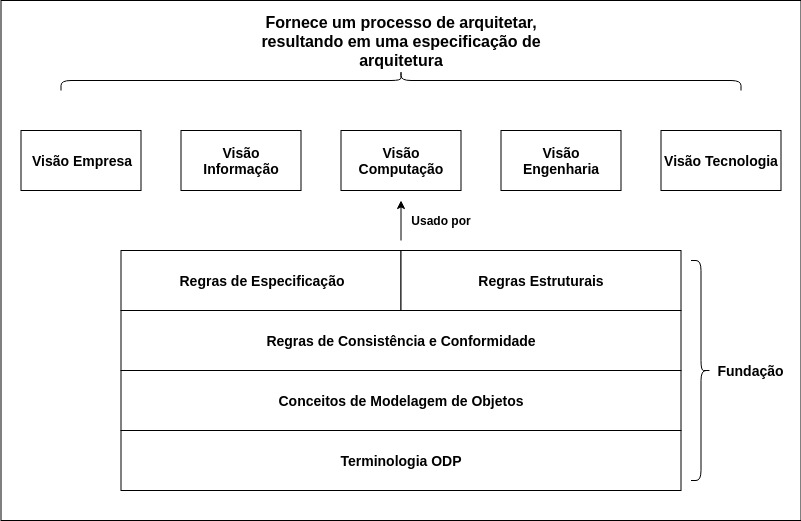
\includegraphics[width=0.9\textwidth]{VisoesRM-ODP}
    \caption*{Fonte: (\citeauthoronline{putman2001architecting}, \citeyear{putman2001architecting})}
    \label{fig:visoes_rmodp}
\end{figure}

\section{Microsserviços}
Microsserviços é uma abordagem para desenvolvimento de uma aplicação como um conjunto de pequenos serviços, onde cada serviço possui seu próprio processamento e possui comunicação com os demais e são construídos em torno das necessidades de negócios do sistema. Os serviços possuem um gerenciamento centralizado enxuto, servindo para poucas tarefas como identificar falhas, rebalanceamento dos serviços e instanciação dos mesmos. Entre as arquiteturas de microsserviços existem características comuns que destacam este modelo de um modelo monolítico, considerando as vantagens e desvantagens (\citeauthoronline{martinfowler2014microservices}, \citeyear{martinfowler2014microservices}).

A divisão de componentes através de serviços é uma das principais características de microsserviços, eles servem como componentes do sistema, cada componente é uma unidade de software independente que pode ser trocada ou melhorada, onde procura minimizar o uso de bibliotecas compartilhadas entre os serviços. Uma consequência de uso de serviços como componentes de um sistema é a necessidade de interfaces mais explícitas para cada serviço e com baixo acoplamento entre os serviços, um dos efeitos negativos dessa abordagem é que as chamadas remotas entre processos são mais custosas e assim devem possuir uma granularidade mais grossa nas \textit{APIs} remotas, evitando congestionamento na rede entre troca de dados constantes entre serviços (\citeauthoronline{martinfowler2014microservices}, \citeyear{martinfowler2014microservices}).

Por possuir uma base de construção dos serviços em torno das necessidades de negócios, cada serviço possui um conjunto maior de implementação da área de negócio, incluindo uma interface com usuário, banco de dados, comunicação externa com outros produtos para cada serviço implementado. Uma consideração nessa abordagem é o cuidado com a quantidade de tecnologias e ferramentas aplicadas em cada serviço, um equilíbrio deve ser considerado a fim de evitar dificuldade de aplicar manutenção sobre os serviços, isso é obtido através de padrões entre projetos e serviços entre as equipes que desenvolvem os serviços (\citeauthoronline{martinfowler2014microservices}, \citeyear{martinfowler2014microservices}).

Seu foco de desenvolvimento é em relação a produtos e não a projetos, sendo que o objetivo de cada equipe esteja direcionado a um produto durante todo seu ciclo de vida, desde o desenvolvimento até sua manutenção, aumentando o contato entre os desenvolvedores e usuários finais. Se destacam também o uso de automatização na infraestrutura de desenvolvimento, tornando possível para as equipes fornecer entregas contínuas (\textit{Continuous Delivery}, CD) e integração contínua (\textit{Continuous Integration}, CI) (\citeauthoronline{martinfowler2014microservices}, \citeyear{martinfowler2014microservices}).

Um dos fatores importante em determinar o quão pequeno deve ser um serviço é considerar o quanto o serviço está alinhado com a estrutura da equipe, se um serviço possui um conjunto de código grande demais para que uma equipe consiga gerenciar, pode ser necessário separá-lo em partes menores, considerando o objetivo de maximizar os benefícios que a arquitetura em microsserviços oferece, de modo que o uso heterogêneo de tecnologias entre os serviços não aumente a complexidade de gerenciamento, a resiliência (tolerância a falhas) esteja em um nível aceitável e sejam pequenos suficientes para que consiga ter escalabilidade quando necessário a partir de cada serviço (\citeauthoronline{Newman}, \citeyear{Newman}).

\begin{figure}[H]
    \centering
    \caption{Princípios do Microsserviços.}
    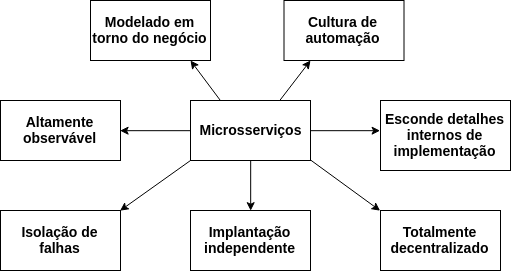
\includegraphics[width=0.8\textwidth]{microservices}
    \caption*{Fonte: (\citeauthoronline{Newman}, \citeyear{Newman})}
    \label{fig:newman}
\end{figure}

\section{Computação em nuvem} \label{comp_nuvem}
Uma das transformações na maneira de fazer computação é utilizá-la como um modelo de serviços que são entregues de uma maneira similar a serviços tradicionais como eletricidade, água e gás. Nesse modelo, usuários acessam os serviços baseado em suas necessidades sem considerar onde os serviços são armazenados e como são entregues. Entre os paradigmas que abordaram essa visão de entregar computação como um serviço está incluso computação distribuída (\textit{Grid Computing}), computação em \textit{cluster} \textit{(Cluster Computing}) e mais recente computação em nuvem \textit{(Cloud Computing}) (\citeauthoronline{Buyya}, \citeyear{Buyya}).
Computação em nuvem, caracteriza pela infraestrutura como uma “nuvem” na qual negócios e usuários são capazes de acessar a partir de qualquer lugar do mundo e além disso sob demanda, a partir disso se obteve a transformação de desenvolver software para milhões de usuários consumirem como um serviço mais do que para usuários executar em seus próprios computadores (\citeauthoronline{Buyya}, \citeyear{Buyya}).

Como uma definição mais formal, dada pelo instituto de padrões NIST,  computação em nuvem é um modelo para possibilitar acessar a uma rede de computadores de recursos de computação compartilhadas de uma maneira ubíqua, conveniente e sob demanda, eles devem ser capazes de rapidamente prover e entregar estes recursos com o mínimo de esforço de gerência e interação com os provedores. O NIST considera para o modelo em nuvem 5 características essenciais,  3 modelos de serviços e 4 modelos de distribuição (\citeauthoronline{nist}, \citeyear{nist}).

As características essenciais são: Serviços sob demanda; Acesso abrangente a rede; Agrupamento de recursos; Rápida elasticidade; e Serviços com métricas. Os serviços devem prover os recursos computacionais conforme a necessidade, sob demanda, sem depender de interações humanas com os fornecedores. Esses recursos devem está disponível pela rede e poderem ser acessados pelos mecanismos padrões de uso e acesso, tais como celulares, notebooks, tablets, garantindo um uso heterogêneo. Os recursos computacionais são agrupados para serem utilizados por múltiplos consumidores, onde componentes físicos e recursos virtuais são dinamicamente atribuídos conforme a demanda do consumidor. Os recursos e serviços devem ser capazes de ser provisionados e desalocados de uma maneira automática, com garantias de rápida escalabilidade. Tais recursos devem possuir métricas que, considerando o tipo de serviço e recurso, possam ser monitorados, controlados e  fornecem uma transparência tanto para o fornecedor do serviço quanto para o consumidor que utiliza (\citeauthoronline{nist}, \citeyear{nist}).

Para os modelos de serviços, é considerado software, plataforma e infraestrutura como serviços a serem oferecidos. No modelo \textit{Software as a Service} (SaaS), o serviço a ser oferecido ao usuário é o uso de aplicações executadas na infraestrutura da nuvem, com fácil acesso e não necessita gerenciar ou controlar níveis abaixo da aplicação como redes, sistema operacional e servidores. No modelo \textit{Platform as a Service} (PaaS), o serviço a ser oferecido ao usuário é a implantação na nuvem de uma infraestrutura criada pelo usuário com o uso de linguagens de programação, bibliotecas e ferramentas, de modo que também não gerencie os níveis abaixo. No modelo \textit{Infrastructure as a Service} (IaaS), o serviço a ser oferecido são os recursos de processamento, armazenamento, rede e outros fundamentais para que o usuário seja capaz de rodar qualquer aplicação, incluindo sistemas operacionais personalizados, uso de \textit{firewalls}, entre outros (\citeauthoronline{nist}, \citeyear{nist}).

Os modelos de distribuição consiste em definir o nível de acesso a nuvem, desde um modelo mais restrito que é uma nuvem privada até o modelo mais permissivo como a nuvem pública. No modelo de nuvem privada, a infraestrutura da nuvem é fornecida exclusivamente a uma única organização, tendo seu gerenciamento pela própria organização ou uma terceira. Em um modelo de nuvem comunitária, seu uso é exclusivo de uma comunidade de consumidores de diversas organizações que tenham em comum os mesmos objetivos, políticas. Na nuvem pública, a infraestrutura é oferecida ao público em geral, seu uso pode ser gerenciado por uma empresa, centros acadêmicos, governos, ou combinações diversas. Além dos citados, existe o modelo híbrido que busca a combinação dos outros modelos com o objetivo de permanecer a usuários distintos mas que utilizem as mesmas tecnologias proprietárias ou padronizadas que permitam a portabilidade de dados e aplicações, tais como balanceamento de carga entre nuvens (\citeauthoronline{nist}, \citeyear{nist}).


\section{IoT (Internet of Things)}
\textit{Internet of Things} (IoT) é um paradigma que pode ser definido como uma interconexão de diversos dispositivos, ou coisas, sobre a Internet, com diversas funcionalidades que permitem medições sobre ambiente, comunicação e execução de uma determinada ação. Existem diversas aplicações para IoT, podendo ser utilizado em um ambiente residencial como uma casa inteligente (\citeauthoronline{iot_kelly}, \citeyear{iot_kelly}), fornecendo reduções de consumo e automatizações de ações como ligar uma lâmpada, bem como pode também ser utilizado em cidades inteligentes, com diversos dispositivos coletando dados, como câmeras, e fornecendo informações úteis para monitoração, administração dos recursos públicos, entre outros.

IoT pode ser definido em 3 categorias, sendo uma internet de pessoa para pessoa, pessoa para máquina ou máquina para máquina. Sendo que a visão do IoT, como conceito e paradgma, considera a presença pervasiva desses dispositivos capazes de interagir entre si e cooperar de forma a criar novos serviços e aplicações que tenham um objetivo em comum. Onde seja possível ter um mundo onde o real, digital e virtual convirjam para criar ambientes cada vez mais inteligentes (\citeauthoronline{iot_patel}, \citeyear{iot_patel}).

Existe um conjunto de características fundamentais que se destacam no IoT. Interconectividade entre os dispositivos, qualquer coisa pode ser interconectada independente do contexto ou localização. Serviços relacionados a coisas,  que consideram as restrições dos dispositivos e impactos relacionados, como a proteção da privacidade,  consistência semântica entre entre coisas virtuais e físicas, entre outros. Heterogeneidade, cada dispositivo se baseia em tecnologias e hardwares distintos, e são capazes de comunicar entre si através de diferentes plataformas e redes. Mudanças dinâmicas e constantes, cada dispositivo pode mudar seu estado (conectado, desconectado, modo de suspensão, etc.) bem como sua localização, velocidade de conexão e quantidade de dispositivos envolvidos. Gerenciamento em grande escala, dado a quantidade de dispositivos conectados e interagindo, existe um grande conjunto de dados sendo trafegado pela Internet. Segurança (Safety), um fator essencial a ser considerado nos dispositivos e em seu processo de comunicação, principalmente aqueles relacionados ao bem-estar (\citeauthoronline{iot_patel}, \citeyear{iot_patel}).

Existem atualmente 5 tecnologias que são amplamente utilizadas para desenvolvimento e comunicação de produtos e serviços baseados em IoT. Identificação por radiofrequência (\textit{Radio frequency identification}, RFID), é uma tecnologia que permite identificação e captura de dados automática através de ondas de rádio, as tags utilizadas no RFID podem ser passivas, quando o leitor provê a energia necessária para transferir o dado, podem ser ativas, quando a tag possui uma bateria integrada e inicia as comunicações com o leitor, ou finalmente, podem ser do tipo semi-passiva, possuindo bateria para o chip interno mas a comunicação é através do leitor. Redes de sensores wireless (\textit{Wireless sensor networks}, WSN), é uma tecnologia que consiste em dispositivos autônomos distribuídos e equipados com sensores que permitem o monitoramento de condições físicas ou do ambiente, permitindo topologias diferentes de redes, com baixo consumo de energia, baixo custo e comunicação \textit{wireless}. \textit{Middleware}, é uma camada de software entre aplicações com o objetivo de facilitar ao desenvolvedores a realização da comunicação e lidar com entradas e saídas das aplicações, seu foco está em esconder os detalhes de diferentes tecnologias. Computação em nuvem que, como comentado na seção \ref{comp_nuvem}, consiste de um modelo de acesso sob-demanda a recursos compartilhados de computadores, redes, servidores, armazenamento, entre outros que são necessários para aplicações IoT que necessitam tomar decisões em tempo real. Aplicações IoT, que permitem interações entre dispositivos e humano para dispositivo de uma maneira confiável e robusta, onde se tem a necessidade de garantir que os dados sejam transmitidos e recebidos em um tempo aceitável.(\citeauthoronline{iot_lee}, \citeyear{iot_lee}).


\chapter{Tecnologias Utilizadas}
\section{YOLO} \label{yolo}
YOLO, acrônimo de \textit{You Only Look Once}, é um sistema de detecção de objetos direcionado para processamento em tempo real. Ele possui uma arquitetura unificada que é extremamente rápida (\citeauthoronline{yolov1}, \citeyear{yolov1}). O sistema possui três versões, YOLO, YOLO9000 e YOLOv3, e vem sendo melhorado incrementalmente ao longo do tempo. Este projeto utiliza a terceira versão do YOLO com um modelo pré-treinado na base de dados \textit{COCO dataset}, sendo capaz de detectar 80 objetos diferentes.

Alguns sistemas de detecção de objetos usam a técnicas como \textit{sliding window} e \textit{region proposal}, onde é preciso rodar diferentes componentes mais de uma vez na imagem ou em partes dela e, adicionar pós processamento para refinar as detecções. Esses pipelines complexos são lentos e difíceis de otimizar, porque cada componente individual deve ser treinado separadamente (\citeauthoronline{yolov1}, \citeyear{yolov1}). O YOLO reformulou a detecção de objetos para um único problema de regressão, onde agora só é preciso olhar uma única vez em uma imagem. Simplificadamente, o processo consiste em redimensionar a imagem de entrada, executar uma única CNN e limitar as detecções com base na confiança (probabilidade de a detecção estar correta) de cada detecção.

Se comparado com outros modelos, o YOLO tem uma performance melhor, seu tempo de resposta chega a ser 3 vezes mais rápido que o SSD (\textit{Single Shot Detector}). Uma de suas variantes (YOLOv3-608) possui uma acurácia alta comparável ao estado da arte em acurácia (modelo \textit{FPN FRCN}) e ainda consegue ter um tempo de resposta baixo (50ms), na Figura \ref{fig:yolo_comparacao}, é mostrado uma comparação das variantes do YOLOv3 em relação aos outros modelos.

\begin{figure}[H]
    \centering
    \caption{Comparação entre os modelos de detecção de objetos utilizando o dataset COCO como benchmark}
    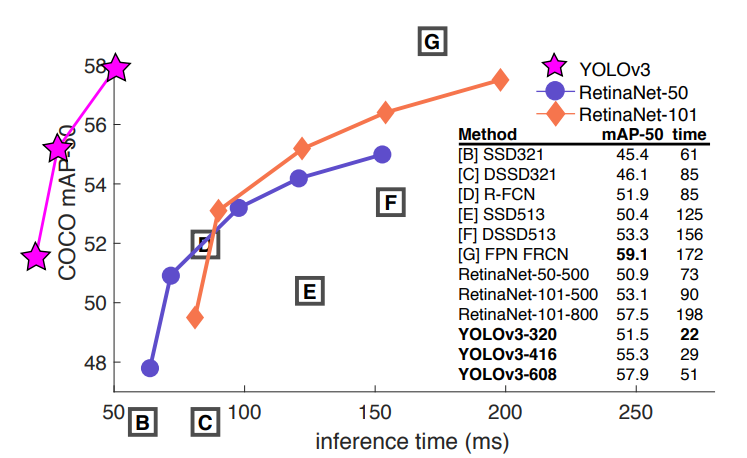
\includegraphics[width=0.8\textwidth]{yolov3_comparacao}
    \caption*{Fonte: (\citeauthoronline{yolov3}, \citeyear{yolov3})}
    \label{fig:yolo_comparacao}
\end{figure}

O YOLOv3 utilizada um CNN de 53 camadas (ver Figura \ref{fig:yolo_arquitetura}) para realizar a extração das características das imagens. Esta arquitetura é uma abordagem baseada no YOLOv2 e outras redes. Ela é significantemente maior que a última versão, porém ainda é eficiente.

\begin{figure}[H]
    \centering
    \caption{Arquitetura da rede neural do YOLOv3}
    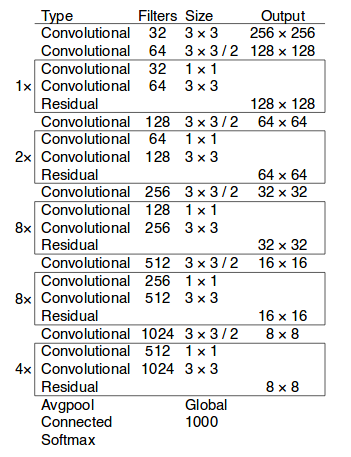
\includegraphics[width=0.5\textwidth]{Arquitetura_YOLOv3}
    \caption*{Fonte: (\citeauthoronline{yolov3}, \citeyear{yolov3})}
    \label{fig:yolo_arquitetura}
\end{figure}

A rede neural recebe uma imagem, cujo tamanho é redimensionado para \(416 \times 416\) pixels. Essa imagem é dividida em uma grade \(N \times N\). Cada célula é responsável por prever apenas um objeto (ver Figura \ref{fig:yolo_grid}), e fornece como saída \(B\) caixas delimitadoras. Cada caixa delimitadora contém cinco componentes, sendo eles, quatro que representam as coordenadas da caixa e um que representa a probabilidade de haver um objeto cujo centro está célula. Além disso, cada caixa fornece a probabilidade condicional de cada classe C, ou seja, a probabilidade de o objeto pertencer a uma certa classe. Assim, as predições são codificadas como \(N \times N \times [B(5+C)]\).

\begin{figure}[H]
    \centering
    \caption{A célula que contém o centro do objeto é responsável por sua detecção}
    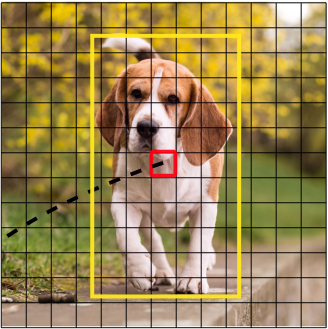
\includegraphics[width=0.7\textwidth]{YOLO_grid}
    \caption*{Fonte: (\citeauthoronline{kathuria}, \citeyear{kathuria})}
    \label{fig:yolo_grid}
\end{figure}

Cada célula fornece como saída B caixas delimitadoras, sendo que as fórmulas apresentadas na Figura \ref{fig:yolo_grid_formula} são utilizadas para transformar a saída da rede em caixas delimitadoras, onde \(b_x\), \(b_y\), \(b_w\) e \(b_h\) são as coordenadas centrais \(x\) \(y\), e largura e altura da caixa, respectivamente, \(t_x\), \(t_y\), \(t_w t_h\) são as saídas da rede, \(c_x\) e \(c_y\) são as coordenadas do topo esquerdo da célula e \(p_x\) e \(p_x\) são dimensões de âncoras para a caixa.

\begin{figure}[H]
    \caption{A célula que contém o centro do objeto é responsável por sua detecção}
    \centering
    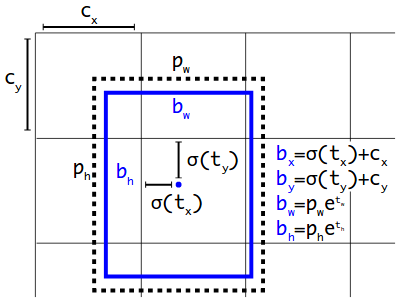
\includegraphics[width=0.6\textwidth]{Bounding_box_dimension_and_location}
    \caption*{Fonte: (\citeauthoronline{yolov1}, \citeyear{yolov1})}
    \label{fig:yolo_grid_formula}
\end{figure}

O YOLOv3 faz predições em 3 escalas diferentes, para deixar a rede menos sensível a escala, sendo elas \(13\times 13\), \(26 \times 26\) e \(52 \times 52\). Além disso, cada célula faz previsões de três caixas, ou seja, \(B=3\), e a base de dados de treinamento contém 80 objetos, ou seja, \(C=80\). Portanto, a rede faz previsões de \([(13 \times 13) + (26 \times 26)+(52 \times 52)] \times 3=10647\) caixas delimitadoras para cada imagem.

Nem todas as 10647 caixas preditas pela rede necessariamente contém um objeto no centro. O primeiro passo para eliminar os resultados irrelevantes é ignorar as caixas cuja probabilidade de haver um objeto sejam menores que um limiar. Para eliminar detecções do mesmo objeto por células adjacentes, usa-se o NMS.

O YOLO impõe grandes restrições espaciais, devido ao fato de cada celular prever um número fixo de objetos. Logo, essa restrição limita a quantidade de objetos próximos na imagem. O treinamento da rede é baseado em uma função de redução de erros, de forma que essa função trata os erros em caixas grandes e pequenas da mesma forma. Um pequeno em uma caixa grande geralmente é inofensivo, mas um erro pequeno em uma caixa pequena gera um grande efeito na IOU. A principal fonte de erros são as localizações incorretas (\citeauthoronline{yolov3}, \citeyear{yolov3}).


\section{OpenCV}
OpenCV (\textit{Open Computer Vision}) é uma biblioteca aberta de visão computacional. Ela foi iniciada na Intel, em 1999, e foi lançada em 2000. Ela é implementada na linguagem C, possui interface para linguagens como C++, Python e Java e está disponível para diferentes plataformas, como Windows, Linux, OS X, Android e iOS. Além disso, as interfaces baseadas em CUDA e OpenCL estão em desenvolvimento ativo para operações de GPU de alta velocidade (\citeauthoronline{opencvtutorials}, \citeyear{opencvtutorials}).

Para auxiliar nas tarefas de processamento de imagens, o OpenCV vem com um conjunto de ferramentas para manipular imagens e vídeos, como ler, gravar, exibir na tela, comprimir, entre outros. Além disso, existem algumas funções para capturar posição do mouse, adicionar textos e formas simples (linhas, retângulos, elipses, círculos, etc) aos quadros.

Na área de processamento de imagens, existem alguns agrupamento de técnicas, onde as principais estão descritas a seguir:
\begin{itemize}
    \item Processamento de imagem: destacam-se os algoritmos de transformações geométricas, extração de gradientes, detecção de bordas, equalização de histogramas e segmentação de imagens
    \item Extração de características: destacam-se os algoritmos de detecção de cantos (e suas variações) e casamento de características
    \item Aprendizado de máquina: destacam-se os algoritmos kNN (\textit{k Nearest Neighbour}), SVM (\textit{Support Vector Machine}) e K-Means \textit{Clustering}
\end{itemize}

\section{ZeroTier}
O ZeroTier é um hypervisor de rede distribuído construído sobre uma rede global \textit{peer-to-peer} criptograficamente segura. Suas principais características consiste em possuir uma virtualização de rede avançada, gerenciamento de recursos como um \textit{switch SDN} e IPSec, servido em redes locais ou globais conectando diversos tipos de dispositivos, como celulares, computadores e equipamentos de rede (\citeauthoronline{zerotier}, \citeyear{zerotier}).

Sua arquitetura consiste virtualização das camadas Ethernet, similar ao modelo VXLAN, porém em uma rede totalmente criptografada. Possui descoberta de vizinhança similar a descoberta de rede da Internet com o DNS, utiliza o conceito de planetas (\textit{planet}) e luas (\textit{moons}) para serem os servidores responsáveis por identificar as mudanças de IPs na rede (\citeauthoronline{zerotier}, \citeyear{zerotier}).

Assim, é possível criar redes privadas com o ZeroTier conectando diversos dispositivos de uma maneira simples, sem preocupar em como irão se conectar, se estão por trás de um NAT (\textit{Network Address Translation}, qualidade do link entre os nós ou qual caminho realizar a comunicação (\citeauthoronline{zerotier}, \citeyear{zerotier}).

\section{Intel Movidius Neural Computer Stick (NCS)}
O \textit{Intel Movidius Neural Computer Stick} (NCS) é um dispositvo dedicado para processamento na área de visão computacional. Este dispositivo conta com uma VPU (Vision Processing Unit), com Intel Movidius Myriad 2, que possui em sua arquitetura uma memória DRAM LPDDR3 de 4Gbits, um microprocessador SPARC (Scalable Processor Architecture) LEON, e 12 processadores SHAVE (Streaming Hybrid Architecture Vector Engine) que é arquitetura híbrida contendo múltiplas unidades funcionais para alto paralelismo e vazão, garantindo em seu design baixo consumo de energia e maximização da performance, como mostrado na figura \ref{fig:intel_movidius}.

\begin{figure}[H]
    \centering
    \caption{Arquitetura da Intel Movidius NCS}
    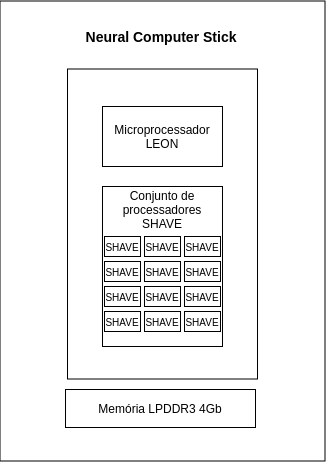
\includegraphics[width=0.45\textwidth]{arquitetura_ncs}
    \caption*{Fonte: (\citeauthoronline{intel_movidius}, \citeyear{intel_movidius})}
    \label{fig:intel_movidius}
\end{figure}

Seu funcionamento consiste em após o dispositivo NCS está conectado, o arquivo com o modelo da rede neural é carregado na memória, o processador LEON executa um \textit{firmware} que é responsável por coordenar o recebimento do arquivo com o modelo da rede neural e imagens para inferência e também cuidar do monitoramento da temperatura. O conjunto de processadores SHAVE recebem os dados processados pelo processador LEON, e realiza as operações de paralelismo, como multiplicação de matrizes. O resultado da rede neural e estatísticas associadas é mandado de volta a máquina que está conectada ao NCS. A comunicação entre o dispositivo NCS e a máquina é feita através da biblioteca NCAPI (Neural Compute API), que cuida da inicialização do dispositivo e carrega o \textit{firmware} necessário para inicializar o recebimento dos arquivos a serem processados.  

Sua aplicação está principalmente na rápida prototipação, validação e desenvolvimento de redes neurais profundas (DNN) em aplicações instaladas em dispositivos. Com sua VPU de baixo consumo, permite que aplicações de inteligência artificial não dependam de conexões com a nuvem, como detecção de objetos a partir de uma câmera. Suporta \textit{frameworks} de desenvolvimento TensorFlow e Caffe, e sistemas operacionais de 64 bits como o Raspberry Pi 3 ou Ubuntu 16.04.


\section{EC2 AWS}

\chapter{Metodologia do Trabalho}

\section{Gerenciamento de tarefas}
Para o desenvolvimento do projeto, foi utilizado a metodologia ágil Scrum, com o objetivo de otimizar o processo de pesquisa e desenvolvimento do trabalho, onde através de Sprints foram definido os ciclos de pesquisa, desenvolvimento e testes do sistema.

Para o controle das entregas, foi utilizado a metodologia Kanbam, através da utilização da ferramenta de gerenciamento online Trello.

\section{Gerenciamento de código}
Para o gerenciamento de código, foi utilizado o sistema de versionamento Git, através da ferramenta online GitHub, para hospedar e versionar os códigos utilizados e desenvolvidos pela equipe.

Cada serviço do sistema foi hospedado em um repositório distinto com instruções de instalação e execução.

\section{Cronograma}
Foi realizado um cronograma inicial, considerando o tempo necessário em cada etapa do trabalho, como é mostrado na Figura \ref{fig:cronograma}.

\begin{figure}[H]
    \centering
    \caption{Cronograma inicial}
    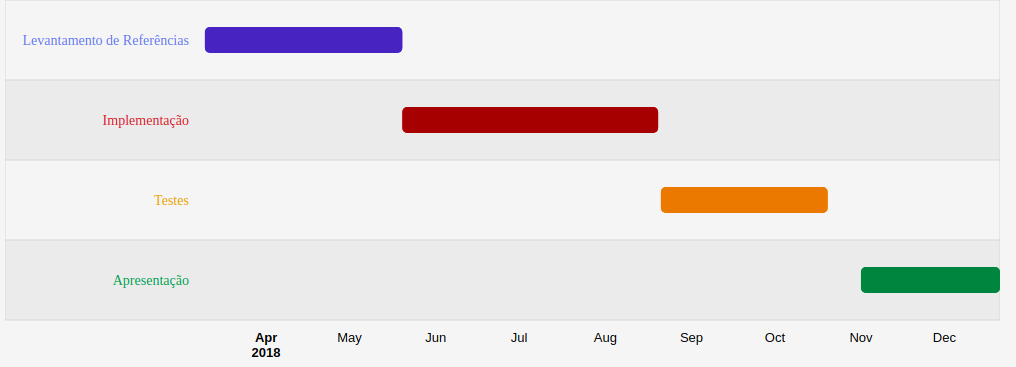
\includegraphics[width=\textwidth]{metodologia_gantt}
    \caption*{Fonte: Autores}
    \label{fig:cronograma}
\end{figure}

\section{Fases do trabalho}
Para o desenvolvimento do trabalho, inicialmente, foi realizado  pesquisas em \textit{papers} e estudos sobre o estado da arte em monitoramento de ambientes, sobre algoritmos de reconhecimento de objetos e aspectos conceituais necessário para o desenvolvimento da monografia. A partir disso, foi elaborado uma arquitetura, afim de atender aos objetivos propostos, na qual maquetes para análise de viabilidade foram feitas para verificar as limitações em relação ao tempo de desenvolvimento e testes da solução a ser proposta. Após essas fases, foi realizado a definição de uma solução técnica com o escopo adequado ao trabalho, e implementado a solução. Com a solução implementada, testes foram realizados para medição dos resultados.

\subsection{Pesquisa}
Entre o conjunto de pesquisas realizadas, foi realizado pesquisas de publicações científicas e industriais na área de monitoramento inteligente, onde pesquisa sobre patentes foram identificadas e produtos que propõem soluções próximas ao nosso objetivo. Foi pesquisado cenários atuais para entender como as câmeras de vigilância estão sendo utilizadas atualmente e quais informações estão sendo extraídas.

Entre os aspectos conceituais importantes para o desenvolvimento da arquitetura, foi pesquisado sobre técnicas de processamento de imagem, \textit{machine learning}, mais especificamente, redes neurais. Para a arquitetura, foi pesquisado e definido o uso do modelo RM-ODP, assim como a abordagem de microsserviços para o desenvolvimento dos módulos do sistema. Entre as tecnologias utilizadas, foi pesquisado sobre computação em nuvem para garantia dos requisitos de escalabilidade do sistema e IoT como forma de coleta da informação necessária do ambiente de atuação. 

Para o algoritmo de detecção de objetos, foram pesquisados técnicas para criar um modelo adequado de detecção de objetos, onde através de ferramentas de \textit{machine learning} como TensorFlow, ser desenvolvido um modelo e treiná-lo para o reconhecimento de objetos, principalmente pessoas em diferentes cenários, atendendo ao requisito de ser um sistema em tempo real. Através de pesquisas, foi identificado a inviabilidade de treinar um modelo do zero no qual atendesse aos requisitos de precisão aceitável para o sistema e que respondesse em um tempo adequado. Nessas pesquisas foi encontrado e selecionado o modelo YOLO, que cumpre com os requisitos de precisão e desempenho especificados pelo sistema.

\subsection{Elaboração da arquitetura}
A primeira etapa para elaboração da arquitetura foi definir os requisitos preliminares, a partir da estruturação do que o sistema precisaria fazer. Com isto foi definido os principais módulos do sistema, como o módulo de coleta dos vídeos, processamento, detecção de eventos e de ações, e a forma de comunicação entre os módulos.



\subsection{Elaboração de maquetes para análise de viabilidade}
Para análise de viabilidade da solução, foram feitos testes de detecção de objetos considerando cenários diversos para a posição da pessoa. Cada cenário consistiu de pessoas em diversos ângulos. Para cada cenário foi verificado a detecção da pessoa e assim garantindo a viabilidade em utilizar o modelo YOLO como base para detecção de objetos e a partir dele desenvolver o algoritmo de detecção de desmaios a partir das pessoas detectadas no vídeo.

\subsection{Definição e implementação da solução técnica}


\subsection{Medição dos resultados obtidos}



\chapter{Especificação do Sistema}
Para especificar o projeto, foi utilizado a visão RM-ODP (Reference Model of Open Distributed Processing), que é estruturada em 5 visões: negócio, informação, computação, engenharia e tecnologia. As seções a seguir contém a descrição de cada uma das camadas.

\section{Visão empresa}
O sistema de Monitoramento Inteligente de Ambientes é um serviço que monitora ambientes, através de vídeos de câmeras de vigilância, detecta eventos relacionados ao bem estar das pessoas presentes no ambiente e presta assistência, quando necessário, realizando um conjunto de ações, em tempo real. Em outras palavras, o sistema recebe vídeos, detecta eventos e realiza ações, visando dar suporte imediato as pessoas contidas nos eventos.

Há uma grande abrangência para os tipos de ambientes, eventos e ações, no contexto do sistema. Os ambientes podem ser do tipo público ou privado, onde os vídeos podem ser provenientes de câmeras de trânsito, monitoramento interno e externo de residências, indústrias, comércios, escolas, hospitais, entre outros. Existem diversos eventos relacionados ao bem estar de pessoas, onde sua detecção pelo sistema se limita pela existência de um algoritmo ou método que seja capaz de detectar tal evento. Alguns exemplos de eventos são: acidente de trânsito, assalto, incêndio, desmaio, agressão física, entre outros. Cada evento necessita de um certo conjunto de ações, que podem ser acionar a polícia, acionar o hospital, acionar corpo de bombeiros, contactar responsável via SMS, chamada de voz ou e-mail, modificar o estado de semáforos de trânsito para isolar áreas, acionar possíveis dispositivos inteligentes para atuar em campo, entre outros.

O sistema conta com três tipos de participantes: clientes, colaboradores e usuários, que podem ser descritos como:

\begin{itemize}
    \item Clientes:
    \begin{itemize}
        \item Poder público: pode utilizar o sistema com a finalidade de aumentar a eficiência na prestação de serviços à população, utilizando seu grande número de câmeras para cobrir áreas públicas;
        \item Particulares: podem utilizar o sistema com vídeos internos e externos, visando aumentar a sensação de segurança de seus clientes;
    \end{itemize}
    \item Colaboradores: são os participantes que contribuem submetendo seus vídeos; eles podem ser atraídos através do oferecimento de bonificações, como prêmios, descontos em lojas, redução no valor de impostos, entre muitos outros;
    \item Usuários: são todos aqueles que estão presentes nos ambientes monitorados pelo sistema.
\end{itemize}

Para que o objetivo do sistema seja alcançado, há um conjunto básico de tarefas que o sistema precisa realizar. Primeiramente, é preciso submeter os vídeos ao sistema, para que seja possível detectar os objetos presentes nas imagens, através de técnicas de visão computacional. Os objetos vão para a fase de detecção de eventos, onde um conjunto de algoritmos analisam os objetos, para detectar os eventos. Os eventos detectados são capturados, onde realiza-se um levantamento do conjunto de ações que é necessário performar para cada evento. Uma vez que o conjunto de ações está definido, realiza-se todas elas.  Para realizar essas tarefas, são necessários os componentes que estão representados esquematicamente pela Figura \ref{fig:componentes}.

\begin{figure}[H]
    \centering
    \caption{Componentes básicos do sistema}
    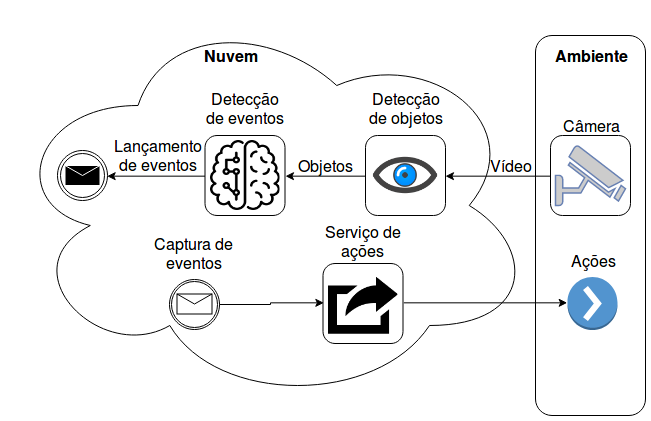
\includegraphics[width=0.7\textwidth]{Componentes_basicos}
    \caption*{Fonte: Autores}
    \label{fig:componentes}
\end{figure}

\section{Visão informação}
O sistema é composto por cinco objetos de dados: Colaborador, Câmera, Vídeo, Evento e Ação. Os colaboradores se cadastram no sistema, para poderem cadastrar suas câmeras. As câmeras transmitem seus vídeos, que são comprimidos e armazenados. Os eventos detectados são registrados, assim como o conjunto de ações tomados.

\begin{figure}[H]
    \centering
    \caption{Diagrama de classes}
    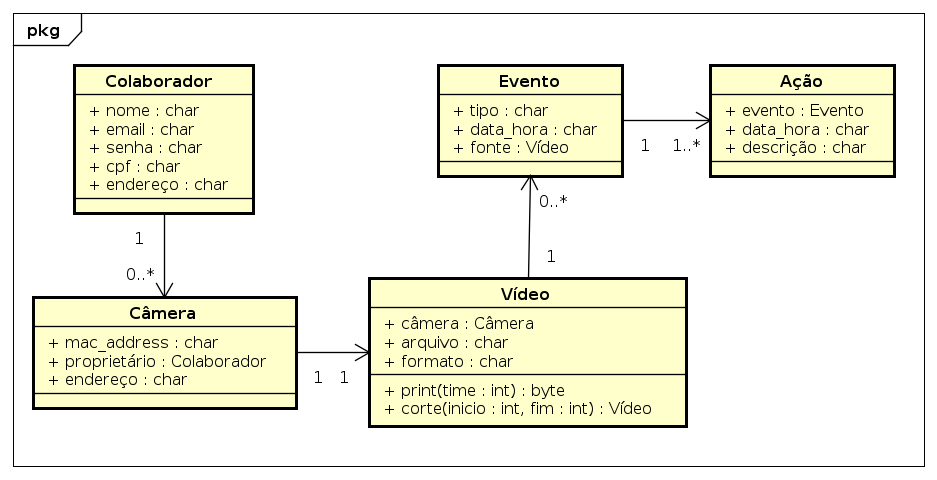
\includegraphics[width=\textwidth]{Visao_informacao_total}
    \caption*{Fonte: Autores}
    \label{fig:classeVisao}
\end{figure}

Existe ainda um pequeno conjunto de dados dinâmicos, que trafegam entre os componentes do sistema, e não são armazenados. A classe Objetos representa os objetos detectados pelo componente de detecção de objetos, que é a entrada do componente de detecção de eventos. A classe Frame representa os quadros do vídeo que são submetidos ao sistema, onde cada quadro deve ter, no máximo, 65 KB, por motivo de desempenho.

\begin{figure}[H]
    \centering
    \caption{Dados dinâmicos}
    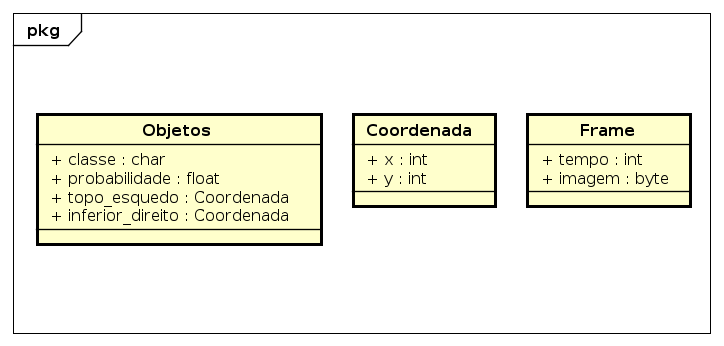
\includegraphics[width=\textwidth]{Visao_info_dinamico}
    \caption*{Fonte: Autores}
    \label{fig:visaoInfomacao_dinamico}
\end{figure}

\section{Visão computação}
Para cumprir com o objetivo proposto, o sistema deve possuir os módulos presentes na \ref{fig:visaoComputacao}. Um dispositivo de submissão de vídeos deve instalado à câmera do colaborador, responsabilizando-se por requisitar permissão e submeter os vídeos de forma privada, confidencial e em tempo real. O módulo de detecção de objetos recebe a requisição de permissão do dispositivo, verifica se o mesmo está cadastrado, alerta o módulo de detecção de eventos, fornece a permissão ao dispositivo e passa a processar, em tempo real, o fluxo de quadros recebidos, detectando os objetos de cada quadro. O módulo de detecção de eventos recebe um alerta do módulo de detecção de objetos, instância os algoritmos disponíveis e passa a processar a lista de objetos contidos em cada frame. O módulo de ações é notificado sempre que um evento é detectado, coletando dados da câmera que gerou o evento e realizando as ações necessárias.

\begin{figure}[H]
    \centering
    \caption{Visão computação}
    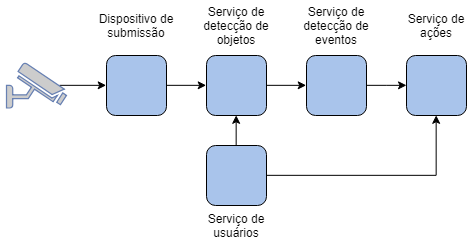
\includegraphics[width=0.8\textwidth]{Visao_Computacao}
    \caption*{Fonte: Autores}
    \label{fig:visaoComputacao}
\end{figure}

Qualquer tipo de participante que queira participar do sistema, precisa se cadastrar. Se o participante for do tipo colaborador, ele poderá cadastrar as câmeras que deseja adicionar.

Uma vez que um dispositivo de submissão é instalado na câmera do colaborador, ele se registra no detector de objetos, informando seu identificador. O detector de objetos verifica a existência desse dispositivo nos registros, e em caso positivo, cria uma instância do modelo que fará as detecções e, emite um alerta ao detector de eventos. Sempre que o detector recebe um alerta, instância os algoritmos disponíveis, para que eles processem o fluxo de objetos que está para chegar. Quando o dispositivo de submissão recebe a permissão, inicia-se o seguinte laço: o dispositivo envia um frame, o detector de objetos detecta os objetos, o detector de eventos processa a lista de objetos.

\begin{figure}[H]
    \centering
    \caption{Diagrama de sequência do processo de submissão de vídeo}
    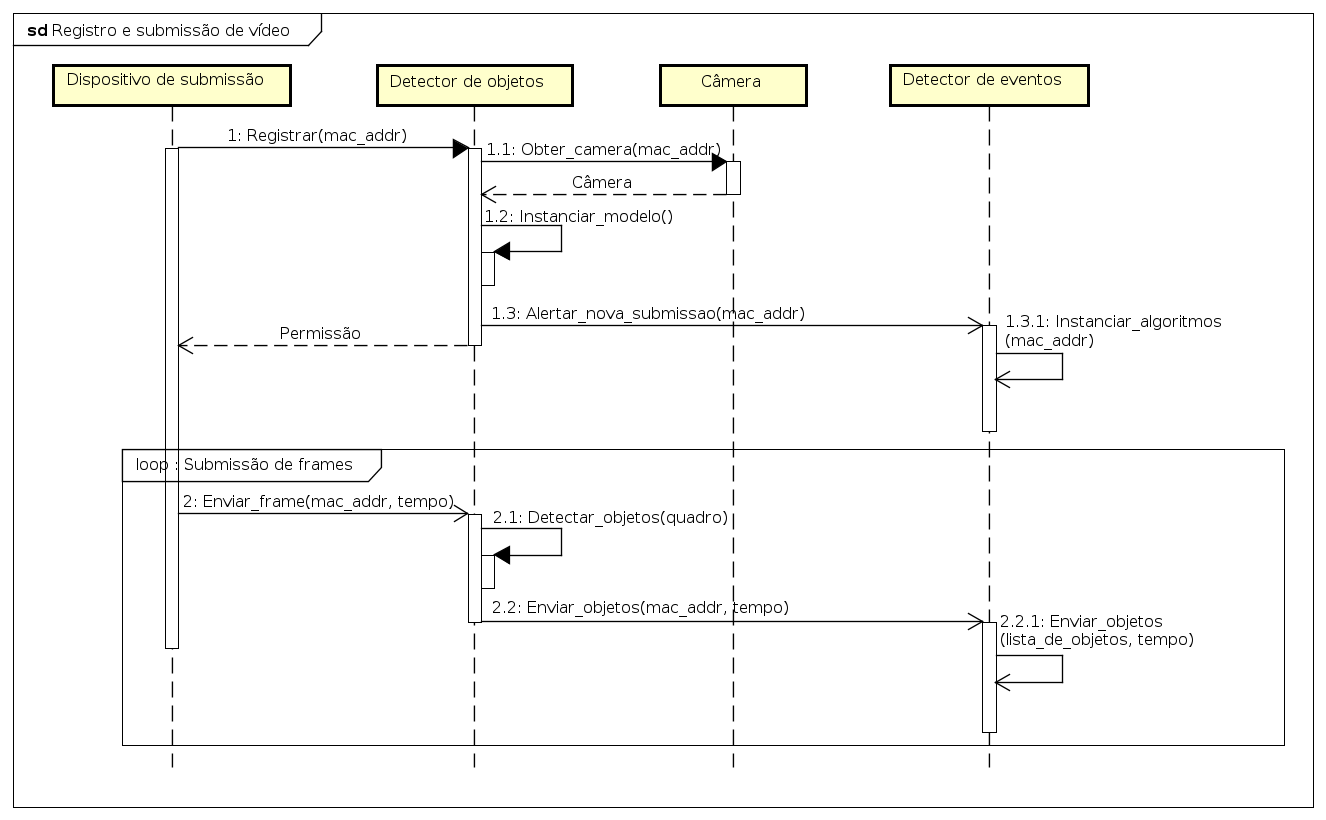
\includegraphics[width=\textwidth]{Registro_e_submissao_video}
    \caption*{Fonte: Autores}
    \label{fig:registro}
\end{figure}

Quando um evento é detectado, o detector de evento alerta ao módulo de ações, informando o identificador do vídeo gerador e o tipo de evento, que, por sua vez, obtém os dados da câmera, calcula quais ações devem ser tomadas, e realiza todas as ações calculadas.

\begin{figure}[H]
    \centering
    \caption{Diagrama de sequência do processo de detecção de evento}
    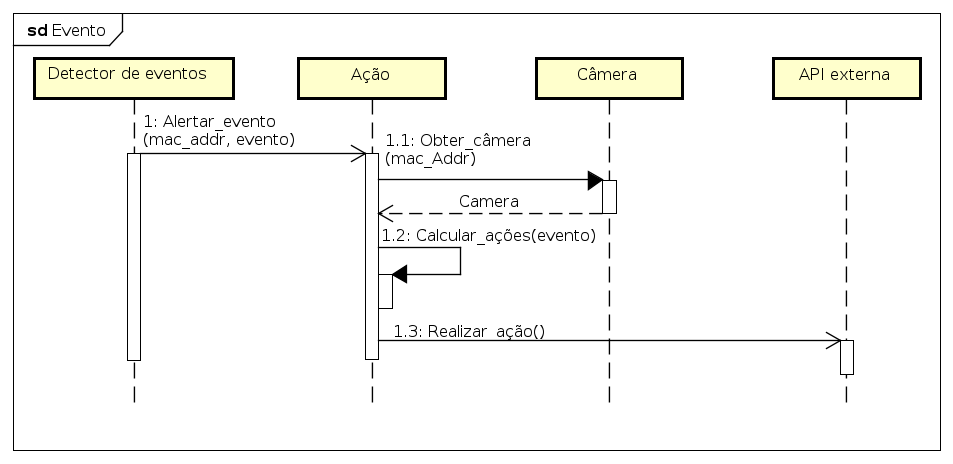
\includegraphics[width=\textwidth]{Evento}
    \caption*{Fonte: Autores}
    \label{fig:evento}
\end{figure}

\section{Visão engenharia}
Esta seção contém a solução arquitetural do sistema, para atender aos requisitos levantados nas visões informação e computação. A visão informação definiu os módulos do sistema, que serão modelados usando a arquitetura de micro serviços. Os micro serviços do sistema são: submissão de vídeo, detecção de objetos, detecção de eventos, ações e usuários.

Para atender aos requisitos de privacidade e confidencialidade, toda a comunicação entre os serviços de sistema são feitos através de VPNs, e estão representados explicitamente nos diagramas.

\subsection{Submissão de vídeo}
Dispositivos de submissão de vídeo são instalados às novas câmeras cadastradas pelos colaboradores. Ao serem ligados, solicitam permissão para submeter seus vídeos ao serviço de detecção de objetos, via protocolo HTTP. Quando recebem permissão, submetem seus vídeos em tempo real, usando o protocolo UDP/IP. 

Para aumentar a disponibilidade, os dispositivos de submissão de vídeo podem detectar falhas no serviço de detecção de objetos, e passam a realizar o processamento localmente, detectando objetos e rodando os algoritmos mais críticos em relação ao bem estar dos usuários. Quando um evento é detectado, ele alerta o serviço de ações por conta própria, via protocolo HTTP.

\begin{figure}[H]
    \centering
    \caption{Arquitetura dos serviços envolvidos na submissão de vídeos}
    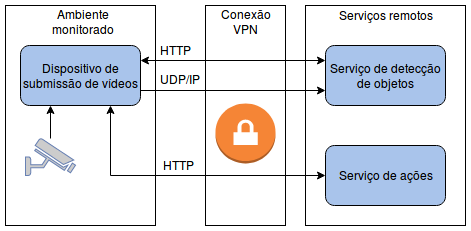
\includegraphics[width=0.8\textwidth]{arquitetura_sub_videos}
    \caption*{Fonte: Autores}
    \label{fig:arquitetura_video}
\end{figure}

\subsection{Detecção de objetos}
Sempre que um dispositivo de submissão de vídeo é iniciado ele solicita permissão para submissão. Para dar a permissão, o serviço de detecção de objetos se comunica, via HTTP, com o serviço de usuários, para verificar se o dispositivo solicitante está cadastrado.

O serviço de detecção de objetos fica constantemente processando todos os quadros recebidos de todas as câmeras, e envia os objetos detectados, no formato JSON, para o serviço de detecção de eventos. Essa troca de dados é assíncrona e utiliza o protocolo MQTT.

\begin{figure}[H]
    \centering
    \caption{Arquitetura dos serviços envolvidos na detecção de objetos}
    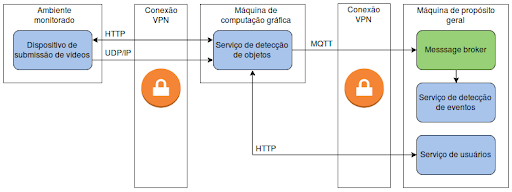
\includegraphics[width=\textwidth]{arquitetura_objetos}
    \caption*{Fonte: Autores}
    \label{fig:arquitetura_objetos}
\end{figure}

\subsection{Detecção de eventos e tomadas de ações}
Quando o serviço de detecção de eventos detecta um evento, ele se comunica, via HTTP, com o serviço de ações, informando o tipo de evento e o identificador da câmera que originou o mesmo. Com essas informações, o serviço de ações coleta dados adicionais, como nome do dono na câmera e endereço, do serviço de usuários, via HTTP. Quando todas as ações tiverem sido calculadas, atua realizando requisições a APIs externas, via HTTPS.

\begin{figure}[H]
    \centering
    \caption{Arquitetura dos serviços envolvidos na detecção de eventos e tomadas de ações}
    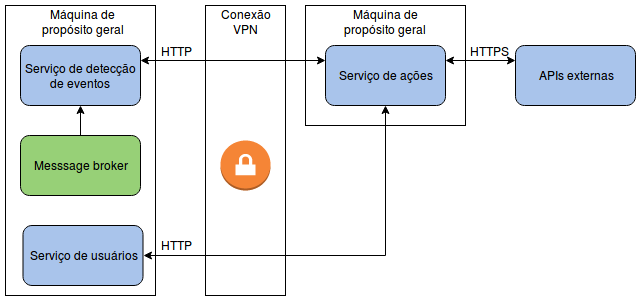
\includegraphics[width=0.8\textwidth]{arquitetura_acoes}
    \caption*{Fonte: Autores}
    \label{fig:arquitetura_acoes}
\end{figure}

\section{Visão Tecnologia}

\subsection{Comunicação}
Os protocolos de comunicação utilizados são:
\begin{itemize}
    \item MQTT, onde utiliza-se a biblioteca Python Paho MQTT para implementar a comunicação e, como mensageiro central, o Mosquitto;
    \item UDP/IP, onde utiliza-se a biblioteca Python Socket, e;
    \item HTTP, onde utiliza-se a própria infraestrutura dos serviços, que são implementados com Django.
\end{itemize}

Para garantir uma comunicação segura, utiliza-se a ferramenta ZeroTier, que cria uma VPN entre as máquinas físicas e oferece uma boa interface de gerenciamento de rede.

\subsection{Serviço de submissão de vídeo}
Para a submissão dos vídeos, o hardware utilizado é um computador single-board, no caso, Raspberry Pi, que é conectado a uma câmera. As principais bibliotecas utilizadas são o OpenCV, para ter acesso à câmera do dispositivo e realizar processamento simples às imagens, como comprimir os quadros e o Paho MQTT para comunicação. Em um dos possíveis cenários, alternativo a mandar o vídeo para nuvem, utiliza para processamento local um Intel Movidius Neural Compute Stick, que se trata de um dispositivo de processamento de visão computacional, executando uma versão Yolo Tiny para a framework Caffe.

\subsection{Serviço de detecção de objetos}
O serviço de detecção de objetos utiliza a \textit{web-framework} Django, para implementar sua interface. Para se comunicar com o serviço de usuários, utiliza-se a biblioteca Python Requests. A recepção de vídeos conta com o uso de Sockets e OpenCV, para descomprimir os quadros recebidos.

O detector de objetos implementa, em Python, a arquitetura de rede neural YOLO, utilizando a biblioteca Pytorch. Este serviço é hospedado nos serviços EC2 da AWS, na família de instâncias “\textit{g3}”, que possui a GPU Tesla M60 e o S.O. Ubuntu Server 16.04 LTS.

\subsection{Serviço de detecção de eventos}
O serviço de detecção de eventos utiliza a \textit{web-framework} Django. A recepção dos objetos detectados nas imagens é feito através da biblioteca Paho MQTT.

\subsection{Serviço de ações}
O serviço de ações utiliza a \textit{web-framework} Django para implementar sua interface. Os registros de eventos tomados são armazenados em banco de dados relacional, utilizando o MySQL. A integração com outras \textit{APIs} é realizada com a biblioteca Requests.

\subsection{Serviço de usuários}
No serviço de usuários foi utilizado Django como \textit{web-framework}, SQLite como banco de dados em ambiente de testes e MySQL no ambiente de produção. Nele é armazenado todas as informações necessárias relacionadas aos usuários e dispositivos cadastrados. O serviço é hospedado nos serviços EC2 da AWS.

\subsection{Ferramentas}
Para desenvolvimento do código, foi utilizado a IDE, para python, PyCharm. Para comunicação entre as máquinas na AWS, o Raspberry Pi e máquinas pessoais foi utilizado ZeroTier, que serve como uma rede virtual, abstraindo problemas de acesso pela Internet.

\section{Requisitos não funcionais}
A partir da análise das visões informação e computação, foi possível extrair os requisitos não funcionais do sistema, onde optou-se por descrevê-los através de tabelas, apresentadas a seguir.

\subsection{Qualidade em uso}
\begin{center}
\begin{longtable}{m{3cm} | m{4cm} | m{4cm} | m{4cm}} 
\caption{\label{tab:qualidade_em_uso}Requisitos de qualidade em uso}\\
\hline\hline
Característica & Sub-característica & Grau & Métrica \\
\hline
\endfirsthead
\caption[]{Requisitos de qualidade em uso (continuação)} \\
\hline
Característica & Sub-característica & Grau & Métrica \\
\hline
\endhead
\hline\hline
\multicolumn{4}{l}{Fonte: Autores} \\
\endlastfoot
\hline
\multicolumn{4}{r}{\footnotesize{}continua na próxima página} \\
\endfoot
Eficácia & Eficiência & Taxa de detecção de eventos de 95\% e taxa de acerto na execução de ações de 99\% & Levantamento de número de falsos e negativos; número de ações não executadas ou incorretas \\ 
\hline
Eficiência & Eficiência & 100\% dos quadros de vídeo devem ser de, no máximo, 65KB. 95\% dos eventos críticos ocorridos devem ser detectados, em, no máximo, 120 segundos & Cálculo do tamanho \\
\hline
Satisfação & Confiança & 90\% dos colaboradores devem concordar com os termos de privacidade & Número de usuários que concordam com os termos de privacidade e aceitam enviar seus vídeos\\
\hline
Isenção de riscos & Mitigação de risco à saúde e segurança & Taxa de falsos positivos menor que 3\% & Levantamento do número de falsos positivos através do relatório gerado pelas autoridades \\
\hline
Cobertura de contexto & Completeza de contexto & O sistema deve detectar eventos em ambientes iluminados (acima de 300 lux), sem chuva, em ambiente rural ou urbano, com resolução tal que a imagem tenha no máximo 65 KB, sem ruídos na imagem, com até 3 pessoas na imagem, de acordo com o requisito de correção funcional & Ambientes iluminado ou não, chuvoso ou não, rural ou urbano, alta qualidade de imagem ou baixa, imagem ruidosa ou não, poucas pessoas na imagem ou muitas devem respeitar o requisito de correção funcional \\
\end{longtable}
\end{center}

\subsection{Qualidade do produto}
\begin{center}
\begin{longtable}{m{3cm} | m{4cm} | m{4cm} | m{4cm}} 
\caption{\label{tab:qualidade_produto}Requisitos de qualidade do produto}\\
\hline\hline
Característica & Sub-característica & Grau & Métrica \\
\hline
\endfirsthead
\caption[]{Requisitos de qualidade do produto (continuação)} \\
\hline
Característica & Sub-característica & Grau & Métrica \\
\hline
\endhead
\hline\hline
\multicolumn{4}{l}{Fonte: Autores} \\
\endlastfoot
\hline
\multicolumn{4}{r}{\footnotesize{}continua na próxima página} \\
\endfoot
 
Adequação funcional & Correção funcional & 5\% a 8\% de falsos positivos e 1\% a 3\% de falsos negativos & Número de falsos positivos e negativos em relação aos eventos detectados\\
\hline

\multirow{2}{3cm}{Eficiência de desempenho} & Comportamento em relação ao tempo & O tempo de detecção de objetos em um quadro deve ser menor que 83,3 ms (12 FPS no mínimo) & Levantamento do número de vezes que a detecção ultrapassou o limite de tempo \\ \cline{2-4}
& Capacidade & O sistema deve suportar o cadastro e submissão simultânea de no mínimo 1,5 milhões de câmeras & Quantidade de câmeras cadastradas no banco de dados e número de vídeos sendo processados \\
\hline

Compatibilidade & Coexistência & Local de instalação deve disponibilizar, no mínimo, 780 Kbps de rede (contando com o uso de outros dispositivos); possuir, no máximo, 5\% de obstrução da câmera e o ambiente não deve possuir iluminação maior que 300 lux na direção da câmera & Número de câmeras submetendo vídeo a menos de 12 FPS; avaliação na hora da instalação das câmeras \\
\hline

Confiabilidade & Disponibilidade & O sistema deve responder a, no mínimo, 95\% dos eventos & Número de vezes que o sistema respondeu, de acordo com a especificação, a um evento \\
\hline

\multirow{2}{3cm}{Segurança de acesso} & Confidencialidade & 0\% dos vídeos privados podem ser acessados por pessoa não autorizada & Número de vídeos visualizados por pessoa não autorizada \\ \cline{2-4}
& Autenticidade & 100\% dos vídeos submetidos devem ser feitos por câmeras autorizadas & Quantidade de vídeos aceitos pelo sistema provenientes de câmeras não autorizadas \\
\end{longtable}
\end{center}

\chapter{Projeto e Implementação}
Uma vez concebida uma ideia de projeto, produto ou serviço, é preciso desenvolver uma arquitetura, para definir as funcionalidade, requisitos e organização de seus componentes. Na fase de implementação, uma etapa importante é definir o escopo, para explicitar quais funcionalidades devem ser implementadas e, quais requisitos devem ser atendidos em cada versão.

\section{Escopo}
A seção 5. define a arquitetura do sistema de forma abrangente, ou seja, como um serviço completo. Este trabalho tem como objetivo implementar as funcionalidades e, atender aos requisitos mínimos necessários para o funcionamento do sistema, para que seja possível provar a viabilidade da ideia proposta.

Os ambientes se restringem aos públicos, como ruas, praças, estações ferroviárias, entre outros. O principal fator para incluir apenas este tipo de ambiente ao escopo está no fato de que não será implementado mecanismos para garantir a confidencialidade, que é um requisito importante para ambientes privados.

Apenas o evento de desmaio será detectado pelo sistema. Este evento está fortemente ligado ao bem estar das pessoas presentes no ambiente, pois, dependendo do motivo que levou ao desmaio, o rápido atendimento pode ser crucial na sobrevivência da vítima.

A ação realizada para o evento de desmaio é o envio de e-mail para um entidade responsável, contendo informações relevantes sobre o evento.

Os participante se restringem apenas a colaborador e usuário. Os colaboradores podem se cadastrar e cadastrar suas câmeras. Não haverá interface para clientes, existindo apenas uma interface de monitoramento do sistema para administradores.

A seção 5.X define todos os requisitos não funcionais do projeto. Com base nesses requisitos não funcionais e com o escopo, a implementação atende todos os itens da Tabela \ref{tab:requisito_nfuncional}.

\begin{center}
\begin{longtable}{m{3cm} | m{4cm} | m{4cm}} 
\caption{
\label{tab:requisito_nfuncional}Tabela de requisitos não funcionais atendidos pela implementação do projeto}\\
\hline\hline
Característica & Sub-característica & Grau \\
\hline
\endfirsthead
\caption[]{Tabela de requisitos não funcionais atendidos pela implementação do projeto (continuação)} \\
\hline
Característica & Sub-característica & Grau \\
\hline
\endhead
\hline\hline
\multicolumn{3}{l}{Fonte: Autores} \\
\endlastfoot
\hline
\multicolumn{3}{r}{\footnotesize{}continua na próxima página} \\
\endfoot
 
Eficiência & Eficiência & 100\% dos quadros de vídeo devem ser de, no máximo, 65 KB. 95\% dos eventos críticos ocorridos devem ser detectados em, no máximo, 120 segundos \\
\hline

Eficiência de desempenho & Comportamento em relação ao tempo & O tempo de detecção de objetos em um quadro deve ser menor que 83,3 ms (12 FPS no mínimo)\\

\end{longtable}
\end{center}

\section{Módulos implementados}
\subsection{Serviço de detecção de objetos}
O serviço de detecção de objetos é a base todo o projeto, de forma que seu correto funcionamento é extremamente importante para os serviços de detecção de objetos e o serviço de ações. Devido sua importância, a detecção de objetos foi o primeiro módulo a ser implementado.

\subsubsection{Módulo de detecção de objetos}
Para implementar o módulo de detecção de objetos, foi utilizada a arquitetura de detecção de objetos YOLO, descrita na seção \ref{yolo}. A implementação oficial da arquitetura foi feita na linguagem C e CUDA, que resultou no framework de código aberto Darknet. A execução do framework dá uma amostra de seu funcionamento, como é possível ver na Figura \ref{fig:dog_yolo}.

\begin{figure}[H]
    \centering
    \caption{Visualização gráfica da execução do \textit{framework} Darknet}
    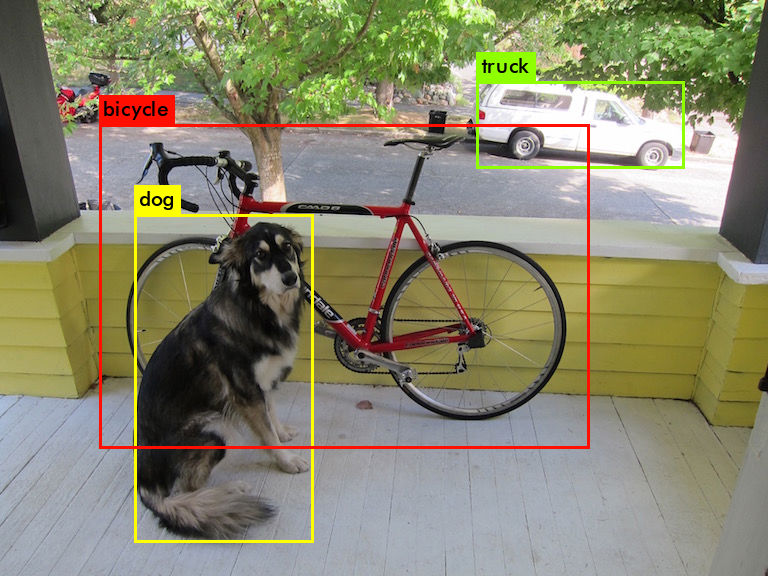
\includegraphics[width=0.7\textwidth]{dog_yolo.jpg}
    \caption*{Fonte: TODO}
    \label{fig:dog_yolo}
\end{figure}

A implementação YOLO utilizada foi a descrita por (\citeauthoronline{kathuria}, \citeyear{kathuria}), que apresenta e detalha a arquitetura da rede neural do YOLO e, como implementá-la utilizando a ferramenta Pytorch, que é uma biblioteca Python para computação científica, muito usada na computação de matrizes e, portanto, possui integração com a biblioteca cuDNN (CUDA Deep Neural Network), que é responsável pelo interfaceamento com a unidade de processamento gráfico (GPU).

Para utilizar essa implementação no projeto, foi preciso criar um interface, onde fosse possível passar imagens como parâmetro e receber a lista de todos os objetos detectados, no formato JSON, para que os algoritmos de detecção de eventos possam consumir esses dados. Com essa interface, a execução do módulo fornece uma saída como a apresentada na Figura \ref{fig:interface_objetos}.

\begin{figure}[H]
    \centering
    \caption{Exemplo de saída da interface do módulo de detecção de objetos}
    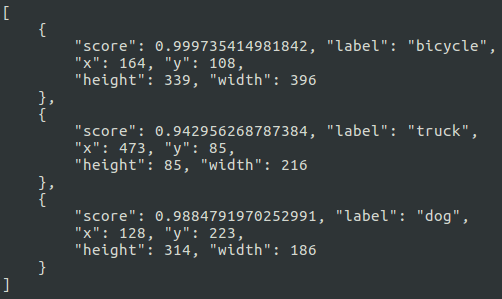
\includegraphics[width=0.8\textwidth]{interface_detector}
    \caption*{Fonte: Autores}
    \label{fig:interface_objetos}
\end{figure}

Devido a variação de iluminação dos ambientes, o módulo aplica a técnica de equalização de histogramas, descrito na seção \ref{histogramas}, utilizando um método presente na biblioteca do OpenCV, que, aumenta o contraste da imagem. Como a detecção de objetos utiliza, em grande parte, informações sobre o contorno dos elementos na imagem, o aumento do contraste ajuda explicitar os contornos, resultando em um aprimoramento na detecção de objetos.

\subsubsection{API}
Para que os outros serviços pudessem utilizar o serviço de detecção de objetos, foi implementado uma API REST, utilizando o web framework Django, conforme os itens a seguir:
\begin{itemize}
    \item \textit{POST}: \textit{register}: método utilizado dispositivos que querem iniciar a submissão de vídeos, onde elas informam seu identificador. O serviço verifica se o dispositivo possui permissão e inicia duas \textit{threads}, uma para receber os quadros e outra para consumir os quadros, realizando a detecção de objetos;
    \item \textit{POST}: \textit{monitor}: método utilizado pela interface do administrador, quando se deseja visualizar o vídeo que algum dispositivo está submetendo;
    \item \textit{POST}: \textit{unregister}: método utilizado para sinalizar que um dispositivo não irá mais submeter seu vídeo;
    \item \textit{GET}: \textit{event\_print}: método utilizado para se obter uma captura do vídeo de um dispositivo específico;
    \item \textit{GET}: \textit{status}: método utilizado para obter o status do sistema, com informações de quantos vídeos estão sendo processados, a taxa de detecção e taxa de recepção de quadros.
\end{itemize}

\subsection{Serviço de detecção de eventos}
O serviço de detecção de eventos é responsável por receber objetos detectados em diversas fontes de vídeos e, detectar os eventos capturados por eles. No escopo do projeto, o evento a ser detectado é o desmaio.

\subsubsection{Comunicação}
Para receber os objetos detectados nas imagens, o serviço utiliza o protocolo MQTT, bastando inscrever-se em um tópico para receber os dados. Toda vez que um dispositivo inicia a submissão de vídeo é criada uma instância do algoritmo de detecção de eventos, para processar especificamente essa fonte de vídeo.

Os algoritmos consomem os objetos detectados em cada frame, e quando detectam um evento, informam o tipo de evento. O serviço obtém a identificação da câmera através da instância que detectou o evento, já que cada instância é atribuída a um fluxo de quadros proveniente de um dispositivo específico. O serviço de ações é alertado via protocolo HTTP, com o auxílio da biblioteca Python, Requests.

\subsubsection{Algoritmo detector de desmaios}
O algoritmo detector de desmaios recebe uma lista com todos os objetos detectados em um quadro, no formato de texto, como exemplificado na Figura \ref{fig:interface_objetos}, e, a partir disso, determina se uma pessoa está desmaiada.

Para este algoritmo, foram classificados três tipos de estados possíveis para uma pessoa: normal, desmaio horizontal e desmaio vertical. Há ainda uma quarta situação, que é o desmaio diagonal, que consiste na combinação linear dos desmaios horizontal e vertical (ver Figura \ref{fig:classes_desmaio}). Observando graficamente algumas detecções nos três estados foi possível identificar alguns padrões e definir as seguintes hipóteses:

\begin{itemize}
    \item Estado normal: a altura da caixa é sempre maior que a largura, ou seja, \(height>width\);
    \item Estado desmaio horizontal: a altura da caixa é sempre menor que a largura, ou seja, \(height<width\);
    Estado desmaio vertical: a largura da caixa varia pouco em relação a largura do estado normal e a altura diminui um certo percentual em relação a altura do estado normal.
\end{itemize}

\begin{figure}[H]
    \centering
    \caption{Categoria de estados: normal, desmaio horizontal, desmaio vertical e desmaio diagonal, respectivamente}
    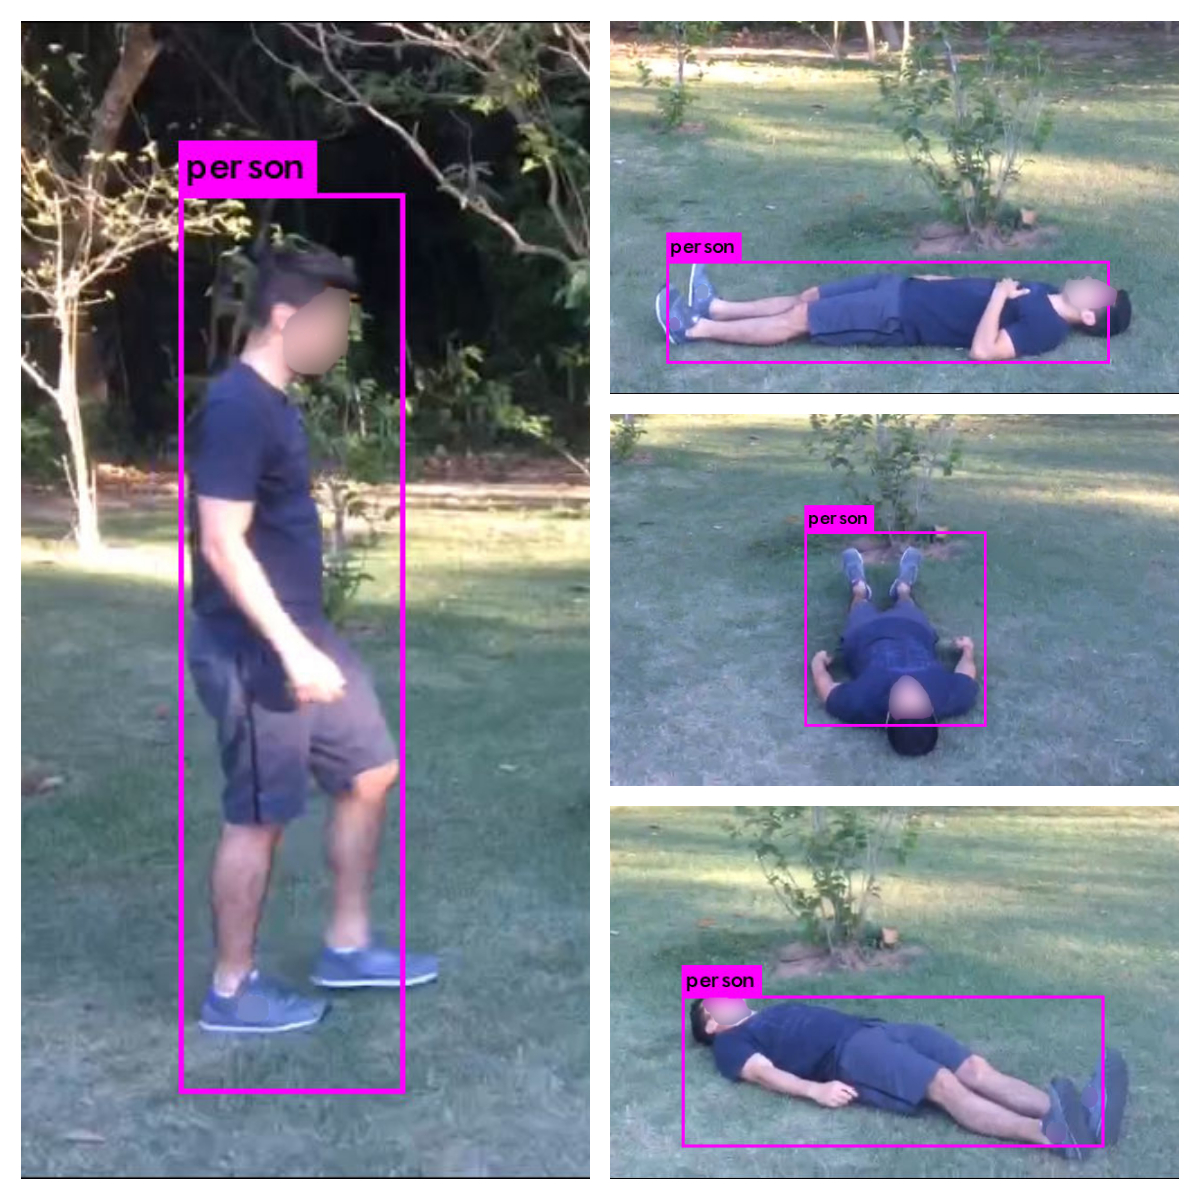
\includegraphics[width=\textwidth]{ClassesDesmaio.jpg}
    \caption*{Fonte: Autores}
    \label{fig:classes_desmaio}
\end{figure}

Dado que \(width\) é a largura e \(height\) é a altura da caixa de detecção, então o estado de desmaio horizontal é atingido quando \(\frac{height}{width}<\alpha\), onde \(\alpha\) é o parâmetro que representa o quanto maior a largura deve ser em relação à altura, e o estado de desmaio vertical, quando \(\frac{height}{highestHeight} < \beta\), onde \(\beta\) é o parâmetro que representa a relação entre altura atual e a maior altura registrada.

Para cobrir possíveis erros, de forma a diminuir os falsos negativos, outra hipótese do algoritmo é que pessoas paradas por muito tempo podem estar com algum problema. Então, se por alguma falha, for atribuído de forma incorreta o estado normal a uma pessoa, quando o correto seria o de desmaio, será detectado falta de movimento, colocando esta pessoa no estado de “sem movimento”. Após um certo tempo neste estado, um alerta é gerado. As imagens que chegam ao detector apresentam pequenas variações na intensidade de cores de alguns pixels, devido à qualidade da câmera e variação da iluminação do ambiente. Então mesmo que os elementos do ambiente não mudem, dois quadros consecutivos tem um pequena, e quase nula, probabilidade de serem idênticos. Este fato, juntamente com erros de precisão do detector, fazem com que a caixa de uma pessoa que não se movimenta de um quadro para o consecutivo tenha variação em sua. Levando em conta esta fato, o conceito de movimento deve levar em conta que mesmo quando a pessoa está parada, sua caixa continua a se mover, através de pequenas oscilações. Portanto, o movimento é definido como a intersecção nula (IoU = 0) entre a última atualização de posição e a posição da caixa atual. Sempre que o movimento é identificado, atualiza-se a posição da pessoa com o valor de posição da caixa que gerou o movimento.

\begin{figure}[H]
    \centering
    \caption{Admite-se movimento quando a intersecção entre a última atualização de posição e a caixa atual é nula}
    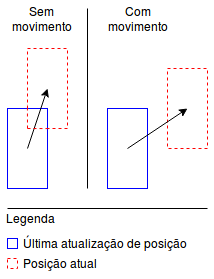
\includegraphics[width=0.5\textwidth]{Movimento}
    \caption*{Fonte: Autores}
    \label{fig:movimento}
\end{figure}

Para eliminar falsos positivos, o algoritmo detecta um estado e apenas gera evento quanto uma pessoa permanece naquele estado por um certo período de tempo, que varia de estado para estado. Quanto maior o tempo esperado, maior é o grau de certeza que se tem de que o estado é verdadeiro, porém, a depender do evento, tempo pode ser um fator crítico, de forma que é preciso obter um compromisso entre grau de certeza e tempo de resposta. Devido aos mesmos ruídos presente nas imagens e erros do detector de objetos, citados anteriormente, algumas detecções não são realizadas, mesmo quando há pessoas na imagem. Essa fato faz com que o histórico da pessoa seja perdido, ou seja, os dado de posição e, principalmente, tempo em um determinado estado sejam perdidos. Suponha que o detector de objetos possua tempo de resposta de 200 ms e taxa de detecção de 90\% e que o tempo necessário para gerar evento de desmaio seja 2 s. Nessas condições, sempre que o evento atingisse tempo de 1,8 s, ocorreria um erro de detecção, levando a perda dos dados, de forma a reiniciar o tempo e posição na próxima detecção corrente. Para contornar esse problema, existe o conceito de persistência, onde os dados de uma pessoa detectada só é excluído após não ser detectado consecutivamente um certo número de vezes.

\subsection{Serviço de ações}
O serviço de ações é responsável por calcular todas as ações cabíveis a um evento e, realizar todas a ações. No escopo de implementação, a ação que deve ser tomada para o evento de desmaio é o envio de um e-mail para um endereço fixo.

Sua API consiste em um único \text{endpoint}, onde o identificador do dispositivo e o tipo de evento são passados como parâmetro. A partir do identificador do dispositivo, são obtidos os dados do mesmo, além de uma captura de imagem do instante do evento. Com essas informações, o e-mail é montado.

A transmissão do e-mail é realizada através da biblioteca Python Boto3, que é uma interface dos serviços SES (\textit{Simple Email Service}) da AWS.

\subsection{Submissão de vídeos}
O serviço de submissão de vídeos é responsável por coletar e enviar o vídeo da câmera ao serviço de detecção de objetos. No escopo de implementação, um Raspberry Pi com uma câmera conectada foi utilizado como dispositivo de coleta, nele é implementado o código de coleta e envio para o serviço de detecção de objetos, através da identificação do dispositivo é solicitado ao detector que fornece uma \textit{thread} para envio do vídeo, caso não consiga após 5 tentativas a solicitação é abortada e notificado.

A transmissão do vídeo é feita através da biblioteca OpenCV para captura da câmera e da biblioteca \textit{Requests} para comunicação. 

\subsection{Serviço de usuários}
O serviço de usuários é responsável por armazenar as informações relacionadas aos usuários do sistema bem como os dispositivos, câmeras, possuídos. Sua API consiste em endpoints que realizam as operações básicas no banco de dados, isto é, adição, busca, edição e remoção de usuários e dispositivos. Está contido nessas informações campos relevantes ao endereço dos usuários e onde estão localizados as câmeras, informações de contato que poderão ser utilizadas no serviço de ações, identificadores únicos tanto dos usuários quanto das câmeras para validação.

\subsection{Dashboard de monitoramento}
O serviço de dashboard de monitoramento é responsável por exibir as informações relevantes aos outros serviços. Entre essas informações consta os logs recebidos dos serviços através do broker MQTT, assim como é possível receber vídeo de depuração do detector de objetos. A sua interface é baseada em um template feito com o framework web Angular, o backend onde é feito as interações com outros serviços utiliza a microframework em python Flask.

\chapter{Testes e Avaliação}
Descrever o procedimento do teste do sistema (teste de hardware, teste de software, teste de módulo, teste de integração, teste de validação), de acordo com o tipo do sistema, com o apoio do orientador, se necessário.


\chapter{Considerações Finais}

\section{Conclusões do projeto de formatura}
\subsection{Em relação ao objetivo declarado}
Apresentar o balanço do trabalho: resultados atingidos e não atingidos, com justificativas.

\subsection{Em relação ao pessoal}
A equipe obteve um aprendizado significativo ao longo da elaboração e desenvolvimento deste trabalho, aplicando métodos e conceitos abordados durante o período de graduação.

Descrever como foi o curso da qual esta se formando....



\section{Contribuições}
Apresentar as contribuições do trabalho, ressaltando o que foi efetivamente da autoria do grupo.

\section{Perspectivas de Continuidade}
Descrever os trabalhos que podem ser realizados como continuação do projeto de formatura.

% \blindtext

% \begin{citacaoLonga}
% 	\blindtext
% \end{citacaoLonga}

% \blindtext

% \blinddocument
% ========== Referências ==========
% --- IEEE ---
%	http://www.ctan.org/tex-archive/macros/latex/contrib/IEEEtran
%\bibliographystyle{IEEEbib}

% --- ABNT (requer ABNTeX 2) ---
%	http://www.ctan.org/tex-archive/macros/latex/contrib/abntex2
\bibliographystyle{abntex2-num}
\bibliography{bibliografia}
% \bibliography{algum item}
% \begin{thebibliography}{5}

% \bibitem{}
% Len Bass, Paul Clements e Rick Kazman. \textit{Software Architecture in Practice}.
% Addison-Wesley, Reading, MA, USA, 2013.

% \bibitem{}
% Lais Giardullo de Araujo, Eric alkmin Santos la Rosa e Saint Clair Barbosa. \textit{Sistema de análise inteligente de vídeo}. Tese de conclusão de curso, Poli, USP, 2017.

% \bibitem{}
% Sergio Sami Saad. \textit{Uma arquitetura de processamento de eventos para gestão de riscos operacionais em ambiente industrial}. Disponível em
% \texttt{http://cassiopea.ipt.br/teses/2013\_EC\_Sergio\_Saad.pdf}. Acesso em: 10 abril 2018.

% \bibitem{}
% OPENCV. Disponível em
% \texttt{https://opencv.org/}. Acesso em: 10 abril 2018.

% \bibitem{}
% Google Cloud Vision API. Disponível em
% \texttt{https://cloud.google.com/vision/}. Acesso em: 10 abril 2018.

% \bibitem{}
% Como funciona um sistema inteligente de monitoramento para indústria. Disponível em
% \texttt{http://www.grupoavantia.com.br/sistema-inteligente-monitoramento-industria/}. Acesso em: 10 abril 2018.

% \end{thebibliography}


% % ========== Apêndices (opcional) ==========
% \apendice
% \chapter{}
% \chapter{Beta}


% % ========== Anexos (opcional) ==========
% \anexo
% \chapter{Alpha}
% \chapter{}



\end{document}
